\documentclass{article}

\usepackage{icomp2026_conference}

\usepackage[T1]{fontenc}
\usepackage[utf8]{inputenc}
\usepackage{tempora}
\usepackage[russian, english]{babel}
\usepackage{hyperref}
\usepackage{url}
\usepackage{booktabs}
\usepackage{nicefrac}
\usepackage{microtype}
\usepackage{xcolor}
\usepackage{amsmath}
\usepackage{cleveref}
\usepackage{subcaption}
\usepackage{graphicx}
\usepackage{multirow}
\usepackage{amsmath,amssymb,amsfonts}
\usepackage{amsthm}
\usepackage{mathrsfs}
\usepackage{textcomp}
\usepackage{manyfoot}
\usepackage{algorithm}
\usepackage{algorithmicx}
\usepackage{algpseudocode}
\usepackage{listings}
\input{math_commands.tex}

\newtheorem{theorem}{Theorem}
\newtheorem{proposition}[theorem]{Proposition}
\newtheorem{corollary}[theorem]{Corollary}
\newtheorem{lemma}{Lemma}
\newtheorem{example}{Example}
\newtheorem{remark}{Remark}
\newtheorem{definition}{Definition}
\newtheorem{assumption}{Assumption}

\algrenewcommand{\algorithmicrequire}{\textbf{Input:}}
\algrenewcommand{\algorithmicensure}{\textbf{Output:}}

\title{The Curious Case of SignMuon: Sign Before or After the LMO?}

\author{
Maria Smirnova\\
  MIRIAI\\
  Moscow, Russia\\
  \texttt{smirnova.m@miriai.org}\\
  \And
  Alexey Kravatskiy \\
  MIRIAI\\
  Moscow, Russia\\
  \texttt{kravatskii.a@miriai.org}\\
}

% \icompfinalcopy

\raggedbottom
\begin{document}

\maketitle

\begin{abstract}\label{sec:abs}
The SignSGD gradient compression algorithm enables up to a $32\times$ reduction in communication volume, which is critical for federated learning in bandwidth-constrained environments. It often lags behind modern optimizers like Muon, which leverage the matrix structure of parameters to achieve superior convergence and performance. We propose SignMuon, an algorithm that applies sign compression to the Linear Minimization Oracle (LMO) update of the Muon optimizer, i.e., it computes $\operatorname{sign}(\operatorname{LMO}(\cdot))$. However, SignMuon offers no global convergence guarantee: we construct a linear function on which SignMuon provably diverges. We complement the counterexample with a descent condition: the sign-compressed LMO step descends whenever the condition number of the gradient is below an explicit threshold determined by the flatness of its polar factor. For generic dense matrices the threshold is an absolute constant, while the divergent instance requires a condition number three orders of magnitude above it; this clarifies why SignMuon performs well in practice. For an unconditional guarantee at the same uplink cost we use EF-USignMuon, an Error-Feedback variant that compresses the residual with $\operatorname{sign}(\cdot)$ and applies the Muon LMO on the server, computing $\operatorname{LMO}(\operatorname{sign}(\cdot))$ while keeping the uplink at one bit per parameter. We prove that EF-USignMuon is an instance of the EF21-Muon framework of Gruntkowska et al.\ (2025) with a contractive (scaled-sign) compressor, and therefore converges at the standard $\mathcal{O}(T^{-1/2})$ rate on smooth non-convex problems; in particular, it converges on the same counterexample. We validate both methods on a synthetic convex problem and on centralized and federated CIFAR-10 classification.
\end{abstract}


% \textbf{Keywords:} federated learning, stochastic optimization, gradient compression, 1-bit quantization, matrix orthogonalization, LMO, SignSGD, Muon.


\section{Introduction}\label{sec:intro}
% Современные методы обучения глубоких нейронных сетей требуют использования оптимизаторов, которые не только обеспечивают высокую скорость сходимости, но и минимизируют коммуникационные издержки в распределенных системах. В условиях федеративного обучения данные распределены между узлами, которые обмениваются информацией с сервером для обучения общей модели. Каждый узел имеет локальный набор данных, а целью федеративного обучения является минимизация усредненной функции потерь по всем узлам. В условиях низкой пропускной способности сети передача полных матриц обновлений модели может замедлять её скорость обучения. Для решения этой проблемы обычно используются методы компрессии градиентов \cite{bernstein2018signsgd,  bernstein2019signsgdmajority, beznosikov2020biased}. 
Modern deep neural network (DNN) training methods require optimizers that not only achieve fast convergence but also minimize communication overhead in distributed systems. In federated learning, data are distributed across clients that communicate with a central server to train a global model. Each client possesses its own dataset and updates its parameters using a local optimizer. The goal of federated learning is to minimize the average loss function across all clients. Under limited network bandwidth, transmitting full model updates can significantly slow down the training process. Gradient compression methods are commonly used to address this issue \cite{bernstein2018signsgd,  bernstein2019signsgdmajority, beznosikov2020biased}.

% Так, алгоритм SignSGD продемонстрировал, что даже экстремальная компрессия (до 1 бита на компоненту) сохраняет работоспособность метода и позволяет сократить объём передаваемых данных примерно в 32 раза при незначительной потере качества модели по сравнению с SGD \cite{bernstein2018signsgd, bernstein2019signsgdmajority}. Однако SignSGD не учитывает матричную структуру параметров: в задачах с матричными весами он рассматривает матрицы как одномерные векторы (flattening), игнорируя их внутреннюю 2D-тензорную структуру, что может ухудшать качество обучения DNN. 
For instance, the SignSGD algorithm has demonstrated that even extreme compression (down to 1 bit per component) can preserve the practical effectiveness of stochastic optimization while reducing the communication volume. This data volume is reduced by a factor of approximately $32\times$ compared to standard SGD, with only minor degradation in model quality \cite{bernstein2018signsgd, bernstein2019signsgdmajority}. However, SignSGD does not account for the matrix structure of the parameters. In tasks with matrix weights, it treats matrices as one-dimensional vectors (flattening), ignoring their intrinsic two-dimensional tensor structure, which may negatively affect the training performance of DNNs.

% Недавно предложенный оптимизатор Muon показал, что его ортонормированные обновления стабилизируют обучение DNN и в ряде случаев превосходят стандартные адаптивные методы оптимизации по качеству итогового решения \cite{jordan2024muon, bernstein2024old, shah2025practical}. Оптимизатор Muon для матричных параметров реализует шаг steepest descent в спектральной норме. Согласно \citet{jordan2024muon}, Muon вычисляет направление обновления как ортонормированную матрицу $\mathbf{U}\mathbf{V}^\top$, где $\mathbf{U}$ и $\mathbf{V}$ -- ведущие сингулярные векторы градиента. Исходя из структуры алгоритма, Muon требует передачи полных матриц обновлений, что в федеративных задачах может быть слишком затратным.  
Recently, Muon has demonstrated that orthonormalized updates can stabilize DNN training and, in several cases, outperform standard adaptive optimization methods in terms of final solution accuracy \cite{jordan2024muon, bernstein2024old, shah2025practical}. For matrix parameters, Muon implements a steepest descent step in the spectral norm. According to \citet{jordan2024muon}, the update direction is computed as the orthonormal matrix $\mathbf{U}\mathbf{V}^{\top}$, where $\mathbf{U}$ and $\mathbf{V}$ are the singular-vector matrices obtained from the gradient decomposition. Based on the structure of the algorithm, Muon requires the transmission of full update matrices, which can be prohibitively computationally expensive for federated tasks.

% В данной работе мы предлагаем алгоритм SignMuon, который применяет знаковую компрессию к LMO-обновлению оптимизатора Muon. В отличие от SignSGD, который передаёт знак координат направления стохастического градиента, наш метод сначала вычисляет направление обновления с помощью LMO (Linear Minimization Oracle), а затем передаёт только знак этого направления. Такая схема позволяет учитывать матричную структуру параметров и сохранять преимущества Muon, одновременно сокращая объём передаваемой информации до одного бита на координату. Тем самым SignMuon стремится объединить быструю сходимость структурированных оптимизаторов с коммуникационной эффективностью знаковых методов.
% In this work, we propose SignMuon,
% % \footnote{Code is available at: \url{https://github.com/intsystems/2026-Project-203/tree/main}},
% an optimization algorithm that applies sign compression to the Linear Minimization Oracle (LMO) update of Muon. SignSGD transmits the sign of the coordinates of the stochastic gradient direction. Our algorithm first computes an update direction using LMO, and then transmits only the sign of this direction. This approach allows for the matrix structure of the parameters to be accounted for and preserves the advantages of Muon, while reducing the amount of transmitted information to one bit per coordinate. Consequently, SignMuon combines the fast convergence of structured optimizers with the communication efficiency of sign-based approaches.
We propose \textbf{SignMuon}, which applies sign compression to the Muon LMO direction: it preserves the matrix-aware geometry of Muon while communicating only one bit per parameter. Empirically, SignMuon matches Muon's accuracy and significantly outperforms SignSGD in both centralized and federated learning.

However, this combination has no global convergence guarantee. We prove (Theorem~\ref{th:1}) that SignMuon can diverge: on a $4\times4$ counterexample, the sign-compressed LMO step becomes an ascent direction. A descent condition (Theorem~\ref{th:descent}) then quantifies how degenerate a problem must be for this to happen: the step provably descends whenever the condition number of the gradient is below an explicit threshold determined by the \emph{flatness} of its polar factor. For generic dense matrices the threshold is an absolute constant, approximately five, whereas the instance of Theorem~\ref{th:1} requires a condition number of $1001$; this clarifies why the divergence, although possible, does not occur on typical problems. For an unconditional guarantee we use \textbf{EF-USignMuon}, obtained by instantiating the EF21-Muon framework of \citet{gruntkowska2025error} with a scaled-sign compressor: each client compresses a gradient \emph{residual} to one bit per parameter, and the server applies the Muon LMO to the reconstructed estimator. We prove that the scaled sign is a contractive compressor (Lemma~\ref{lem:signcontr}), so the framework's guarantee transfers: EF-USignMuon converges at the standard $\mathcal{O}(T^{-1/2})$ rate on smooth non-convex problems (Theorem~\ref{th:conv}), and in particular on the counterexample, while retaining one-bit uplink communication.

% Эффективность предложенного оптимизатора показана на различных синтетических и прикладных задачах: 
% The effectiveness of the proposed optimizer is evaluated on synthetic and practical tasks: centralized image classification on CIFAR-10 with a ResNet-18 backbone, federated image classification on CIFAR-10 with a CNN across several client counts, and on a synthetic smooth convex least-squares problem.
% Наши эксперименты направлены на изучение того, насколько эффективно можно сочетать структурированные направления обновления Muon с экстремальной коммуникационной компрессией знаковых методов. В частности, мы анализируем, как передача только знака направления обновления влияет на качество и устойчивость обучения по сравнению с использованием полного Muon-обновления.
Our experiments investigate how effectively Muon-style structured update directions can be combined with the extreme communication compression characteristic of sign-based methods. Specifically, we analyze how transmitting only the update direction signal affects the accuracy and stability of training compared to using the full Muon update. We validate both methods on centralized image classification on CIFAR-10 with a ResNet-18 backbone, federated image classification on CIFAR-10 with a CNN across several client counts, and on a synthetic smooth convex least-squares problem. Our contributions are:
(i)~SignMuon, a matrix-aware 1-bit optimizer, together with a counterexample (Theorem~\ref{th:1}) proving that it may diverge;
(ii)~a descent condition (Theorem~\ref{th:descent}): ascent requires the condition number of the gradient to exceed an explicit threshold that increases with the flatness of its polar factor, which identifies a class of problems on which SignMuon provably descends;
(iii)~a convergence guarantee (Theorem~\ref{th:conv}) for EF-USignMuon at one uplink bit per parameter: the EF21-Muon framework of \citet{gruntkowska2025error} instantiated with a scaled-sign compressor -- our contribution is the choice of the one-bit compressor and the proof of its contractivity, not a new algorithmic mechanism.

% Экспериментальные результаты показывают, что использование знаковой компрессии для направлений Muon позволяет снизить коммуникационные издержки (в 32 раза), сохраняя при этом темпы оптимизации. В централизованном сценарии алгоритм SignMuon превосходит базовый метод SignSGD по скорости сходимости и итоговой точности. При этом точность предложенного 1-битного метода уступает оптимизатору Muon всего на $1-1.5\%$, при этом уверенно превосходя базовые знаковые алгоритмы. В федеративном сценарии интеграция SignMuon с механизмами клиентского моментума и мажоритарного голосования (Majority Vote) обеспечивает стабильную сходимость и защиту от аномальных обновлений даже в условиях жесткого ограничения пропускной способности сети. Также, в работе представлен аналитический пример, который формализует границы применимости знаковой компрессии к LMO-обновлениям в детерминированном случае и решение гладкой выпуклой задачи. В результате проведенных экспериментов, предложенный подход демонстрирует, что LMO-основанные методы могут быть успешно объединены с знаковой компрессией без существенной потери качества обучения.
% Experimental results show that applying sign compression to Muon directions reduces communication overhead (by $32\times$) while maintaining optimization rates. In the centralized setting, SignMuon consistently outperforms the baseline SignSGD method in both convergence speed and final accuracy. At the same time, the accuracy of the proposed 1-bit method is only $1-1.5\%$ lower than that of the Muon optimizer, while significantly outperforming basic signed algorithms. In federated setting, integrating SignMuon with client momentum and Majority Vote aggregation method provides stable convergence and robustness to anomalous client updates even under severe communication constraints. Furthermore, we present an analytical example that formalizes the limitations of applying sign compression to LMO-based updates in the deterministic setting and for smooth convex optimization problems. The results of our experiments demonstrate that the proposed algorithm successfully combines LMO-based methods with sign compression without any significant loss in training accuracy.

\section{Related Work}\label{sec:relWork}
\paragraph{SignSGD.} Vanilla SignSGD, introduced by \citet{bernstein2018signsgd} and later applied to federated learning by \citet{bernstein2019signsgdmajority}, required increasing batch sizes to guarantee convergence. This issue, together with SignSGD's inherent bias, was addressed through the adoption of the Error Feedback technique \citep{karimireddy2019efsign}. An alternative approach is to randomize the sign operator itself \citep{chen2020median,safaryan2021ssdm,jin2024stosign}.

\paragraph{Compression for Muon.} \citet{gruntkowska2025error} developed a theoretical framework for federated learning with error feedback in which Muon/Gluon \citep{riabinin2025gluon} updates are compressed bidirectionally (client-to-server and server-to-client). Our EF-USignMuon is an \emph{application} of this framework: we instantiate EF21-Muon with the one-bit scaled-sign compressor and verify that this compressor meets the framework's contractivity requirement (Lemma~\ref{lem:signcontr}), after which its analysis applies (Theorem~\ref{th:conv}). \citet{qian2026communicationefficientgluon} employed variance reduction to lower the compression error for Gluon under unbiased and contractive compressors. Concurrently with our work, \citet{mishra2026signmuon} proposed vanilla SignMuon and demonstrated its empirical feasibility, but did not identify an instance of SignMuon's non-convergence such as the one given in Theorem~\ref{th:1}.

\section{Problem Statement}\label{sec:proState}

\paragraph{Centralized Learning:} We consider the stochastic optimization problem:
\begin{equation}
\min_{\mathbf{X} \in \mathcal{X}} \{f(\mathbf{X}) := \mathbb{E}_{\xi \sim \mathcal{D}} [f_{\xi}(\mathbf{X})]\},
\end{equation}
where $\mathcal{X}$ is the parameter space (e.g., $\mathbb{R}^d$ or $\mathbb{R}^{m \times n}$), functions $f_{\xi} : \mathcal{X} \to \mathbb{R}$ are continuously differentiable (possibly non-convex). Here, $f_{\xi}(\mathbf{X})$ is the loss function of a model parameterized by $\mathbf{X}$, computed at a data point $\xi$, sampled from the probability distribution $\mathcal{D}$.

\paragraph{Federated Learning:} 
% В современном мире машинное обучение развивается благодаря масштабированию систем. Сегодняшние передовые модели опираются на массивные наборы данных и сложные архитектуры, требующие большого времени обучения. В современных реалиях задача обучения формулируется как поиск минимума в распределенной среде:
Modern models rely on large datasets and complex architectures, so training is often formulated as an optimization problem in a distributed environment:

\begin{equation}
\min_{\mathbf{X} \in \mathcal{X}} \left\{ f(\mathbf{X}) := \frac{1}{N}\sum_{j=1}^N f_j(\mathbf{X})\right\}, \quad f_j(\mathbf{X})=\mathbb{E}_{\xi_j\sim\mathcal{D}_j}[f_j(\mathbf{X};\xi_j)]
\label{fed_eq}
\end{equation}
where $\mathbf{X} \in \mathcal{X}$ are the model parameters, $N \ge 1$ is the number of clients, and $f_j(\mathbf{X})$ is the loss of the model $\mathbf{X}$ on the data $\mathcal{D}_j$, stored on client $j \in [N] := \{1, \dots, N\}$. In federated learning, clients do local computations and synchronize with a global server. Since communication bandwidth is often limited, the volume of transmitted data becomes a major bottleneck in the training process \cite{bernstein2019signsgdmajority, horvath2023stochastic}. Several practical techniques for federated optimization and communication compression have also been studied in \cite{beznosikov2020biased, gruntkowska2025error, ahn2025dion}.

% Для теоретического анализа оптимизации в таких распределенных условиях мы опираемся на предположение об $L$-гладкости функции $f$ в неевклидовом пространстве, оснащенном нормой $\|\cdot\|$. Формально это означает, что для любых $\mathbf{X}, \mathbf{Y} \in \mathbb{R}^d$ выполняется:
For theoretical optimization analysis in distributed environments, we rely on Assumption~\ref{as:2} that the objective function $f$ is smooth w.r.t.\ the spectral norm. 
% Formally, for any $\mathbf{X}, \mathbf{Y} \in \mathbb{R}^d$, the following condition holds:
% \begin{equation}
% \|\nabla f(\mathbf{X}) - \nabla f(\mathbf{Y})\|_* \leq L \|\mathbf{X} - \mathbf{Y}\|,
% \end{equation}
% where $\|\cdot\|_*$ is the dual norm defined by $\|\mathbf{X}\|_* := \sup_{\|\mathbf{X}'\| \leq 1} \langle \mathbf{X}, \mathbf{X}' \rangle$ \cite{kovalev2025understanding}. 
% В свою очередь, жесткие ограничения на пропускную способность сети делают передачу полных 32-битных градиентов неэффективной. Исходя из этого, в данной работе целесообразно рассмотреть сценарии с экстремальной компрессией, где целевой уровень сжатия составляет 1 бит на компоненту сообщения 
Limited network bandwidth makes the transmission of full-precision 32-bit gradients expensive, motivating optimization methods built on extreme gradient compression \cite{bernstein2018signsgd, bernstein2019signsgdmajority, beznosikov2020biased}.

\textbf{Linear Minimization Oracle (LMO)} is defined as an operator  $A(\cdot)$ that provides the solution to a linear minimization problem over a feasible set. In particular, the constraints can be defined via the unit ball of a given norm:
\begin{equation}
A(\mathbf{X})=\arg\min_{\mathbf{Y} \in \{ \mathbf{Y} \in \mathcal{S} | \|\mathbf{Y}\| \le1\}}\langle \mathbf{X}, \mathbf{Y}\rangle,
\end{equation}
where $\mathbf{X}\in\mathbb{R}^{m\times n}$ is the input matrix, $\mathcal{S}\subset\mathbb{R}^{m\times n}$  is a convex set, and $\langle \mathbf{X},\mathbf{Y}\rangle=\sum_{i,j}{X}_{ij}{Y}_{ij}$ is the standard matrix inner product \cite{pethick2025training}. 

Such an operator selects the direction of steepest descent with respect to the specified norm. The analytical and practical role of the LMO is discussed in detail in the literature on norm-constrained LMO optimizers \cite{pethick2025training, kovalev2025understanding, riabinin2025gluon}.

\textbf{Muon optimizer} uses the matrix structure of the gradient. Muon implements a steepest descent step in the spectral norm, where the update direction is obtained by orthogonalizing the gradient matrix  \cite{bernstein2024old}. Let $\mathbf{M}=\mathbf{U}\boldsymbol{\Sigma}\mathbf{V}^\top$ be the singular value decomposition (SVD) of the matrix $\mathbf{M}\in\mathbb{R}^{m\times n}$, where $\mathbf{U}\in\mathbb{R}^{m\times r}$ and  $\mathbf{V}\in\mathbb{R}^{n\times r}$ are the orthonormal matrices of singular vectors, $\boldsymbol{\Sigma}\in\mathbb{R}^{r\times r}$ is the diagonal matrix of singular values, and $r=\mathrm{rank}(\mathbf{M})$. Then, the LMO direction takes the following form:
\begin{equation}
A(\mathbf{M})=-\mathbf{U}\mathbf{V}^\top \in \mathbb{R}^{m\times n}.
\end{equation}
That is, Muon selects an orthonormal update direction corresponding to the solution of the linear minimization problem induced by the spectral norm geometry. In practice, Muon utilizes a smoothed gradient estimate with momentum, and its update is defined as follows: 
\begin{equation}
    \begin{aligned}
        \mathbf{M}_t &= \mu \mathbf{M}_{t-1} + \mathbf{G}_t, \\
        \mathbf{M}_t &= \mathbf{U}_t \boldsymbol{\Sigma}_t \mathbf{V}_t^\top, \\
        \mathbf{D}_t &= -A(\tilde{\mathbf{M}}_t) = \mathbf{U}_t\mathbf{V}_t^\top\\
        \mathbf{X}_{t+1} &= \mathbf{X}_t - \eta_t \mathbf{D}_t.
    \end{aligned}
\end{equation}

In the original Muon implementation, the computation of $\mathbf{U}_t\mathbf{V}_t^\top$ is approximated using Newton-Schulz iterations and related polynomial schemes. It enables efficient matrix orthogonalization without an explicit SVD computation \cite{amsel2025polar, li2025note, liu2025muon}. Such orthogonalization produces more isotropic updates and prevents a small number of dominant singular directions from controlling the optimization process, which is particularly beneficial for training DNN \cite{bernstein2024old, shah2025practical}.

% Despite its theoretical and practical advantages, Muon requires transmitting the full orthogonalized update matrix $\mathbf{D}_t$. This step makes Muon more expensive in federated learning settings. Our objective is to develop a communication-efficient optimization algorithm, that preserves the geometric properties of Muon's LMO-based updates while reducing the communication cost to the level of SignSGD (1 bit per parameter). At the same time, the proposed method should retain the standard convergence guarantees for smooth non-convex optimization:
% \begin{equation}
% \min_{0 \le t \le T}\mathbb{E}\bigl[\|\nabla f(\mathbf{X}_t)\|_*^2\bigr] = \mathcal{O}(T^{-1/2}).
% \end{equation}
Despite its advantages, Muon requires transmitting the full update matrix $\mathbf{D}_t$, making it expensive in federated settings. Our objective is to combine Muon's matrix-aware geometry with extreme (1-bit) communication compression. SignMuon achieves this combination empirically, but, as we show (Theorem~\ref{th:1}), it lacks global convergence guarantees; Theorem~\ref{th:descent} then gives a lower bound on the condition number of the gradient that is necessary for descent to fail. The Error-Feedback variant EF-USignMuon restores convergence unconditionally: by reduction to the EF21-Muon framework of \citet{gruntkowska2025error} (Theorem~\ref{th:conv}, proved in Appendix~\ref{app:hyp}), it attains the standard rate for smooth non-convex optimization,
\begin{equation}
\min_{0 \le t \le T}\mathbb{E}\bigl[\|\nabla f(\mathbf{X}_t)\|_*^2\bigr]
= \mathcal{O}(T^{-1/2}).
\end{equation}


\section{Theory}\label{sec:theory}
% Рассмотрим семейство алгоритмов SignA, где A обозначает любой оптимизатор, использующий LMO-направления. Все алгоритмы семейства построены по единой структуре, состоящей из трёх последовательных этапов: обработка моментума, вычисление LMO-направления и знаковая компрессия обновления.
Consider the SignA family of algorithms, where A denotes any optimizer based on LMO directions. All methods in this family follow the same three-stage structure: momentum accumulation, computation of an LMO direction, and sign-compression of the resulting update.

Formally, a SignA method initializes the momentum buffer as $\mathbf{M}_0 = \mathbf{0}$, and at each iteration $t \ge 1$ performs the following sequence of updates:
\begin{equation}
\begin{aligned}
\mathbf{M}_t &= \mu \mathbf{M}_{t-1} + \mathbf{G}_t && \text{(Momentum accumulation)}\\
\tilde{\mathbf{M}}_t &= 
\begin{cases} 
    \mathbf{G}_t + \mu \mathbf{M}_t & \text{(Nesterov momentum)}, \\
    \mathbf{M}_t & \text{(otherwise)}
\end{cases} && \text{(Effective direction)}, \\
\mathbf{D}_t &= -A(\tilde{\mathbf{M}}_t), && \text{(LMO direction)} \\
\mathbf{s}_t &= \operatorname{sign}(\mathbf{D}_t) \in \{\pm 1\}^{m \times n},  && \text{(Sign compression)}\\
\mathbf{X}_{t+1} &= \mathbf{X}_t - \eta_t \lambda_{\mathrm{mult}} \mathbf{s}_t && \text{(Parameter update)},
\end{aligned}
\label{eq:signa_general}
\end{equation}
where $\mathbf{X}_t \in \mathbb{R}^{m \times n}$ is the current model parameter matrix, $\mathbf{G}_t$ is its stochastic gradient, $\mu \in [0, 1)$ is the momentum coefficient, $\eta_t$ is the learning rate, and $\lambda_{\mathrm{mult}} > 0$ is an optional scaling factor (with $\lambda_{\mathrm{mult}}=1$ by default). The operator $A(\cdot)$ denotes a Linear Minimization Oracle (LMO) in a specified non-Euclidean norm, and the function $\operatorname{sign}(\cdot)$ is applied element-wise to the resulting structured direction $\mathbf{D}_t$.

% Предлагаемый в работе метод SignMuon является частным случаем класса алгоритмов SignA, он объединяет ортогонализованные LMO-направления оптимизатора Muon с экстремальной знаковой компрессией SignSGD. Ниже описаны две основные реализации данного алгоритма -- централизованная и федеративная.
The proposed SignMuon algorithm is a particular instance of the SignA family. It combines the orthogonalized LMO directions of the Muon optimizer with the extreme sign-based compression strategy of SignSGD. In the following sections, we present SignMuon and EF-USignMuon, each in centralized and federated variants.

\subsection{Centralized Learning}
% В централизованной постановке алгоритм SignMuon применяется к матричным параметрам модели. Практическая реализация алгоритма учитывает тензорную структуру параметров нейронной сети. Процесс оптимизации разделен на два потока: матричные параметры (веса сверточных и полносвязных слоев, $n_{dim} \ge 2$) обновляются с помощью LMO-алгоритма SignMuon, а векторные параметры (bias, Batch Normalization layer, $n_{dim} = 1$) и последний слой классификатора оптимизируются стандартным методом AdamW. Первоначально такой подход был предложен в эмпирическом описании \cite{jordan2024muon}. Первый результат о теоретической сходимости был получен Li и Hong, которые проанализировали гладкую невыпуклую постановку \cite{li2025note}, а также формализован в рамках фреймворка Gluon \cite{riabinin2025gluon}.
% In the centralized setting, SignMuon is applied to the matrix-valued parameters of a neural network. The practical implementation takes into account the tensor structure of model parameters. The optimization process is divided into two separate streams: matrix parameters (weights of convolutional and fully connected layers, $n_{dim} \ge 2$) are updated using the SignMuon LMO-based procedure, whereas vector parameters (bias, Batch Normalization layer, $n_{dim} = 1$) as well as the final classification layer are optimized using the standard AdamW optimizer. This design was originally introduced in the empirical description of Muon by \citet{jordan2024muon}. The first theoretical convergence result was derived by Li and Hong, who analyzed the smooth non-convex setting \cite{li2025note} and subsequently formalized within the Gluon framework \cite{riabinin2025gluon}.
In the centralized setting, SignMuon is applied to the matrix-valued parameters (weights of convolutional and fully connected layers, $n_{dim}\ge 2$), while vector parameters (biases, BatchNorm, $n_{dim} = 1$) and the final classification layer are optimized with AdamW -- the design introduced by \citet{jordan2024muon} and formalized in \cite{li2025note, riabinin2025gluon}.

% Для матричных параметров ключевым этапом алгоритма SignMuon является поиск ортонормированного LMO-направления $\mathbf{D}_t \approx \mathbf{U}_t \mathbf{V}_t^\top$. Чтобы избежать высоких вычислительных затрат на явное вычисление сингулярного разложения (SVD) на каждом шаге оптимизации, на практике применяется итерационный алгоритм Ньютона-Шульца 5-го порядка. В ортогонализации Ньютона-Шульца мы приняли коэффициенты равными $a=3.4445, b=4.7750, c=2.0315$. Отличие нашего подхода от классического SignSGD заключается в том, к какому объекту применяется компрессия. Если в SignSGD знаковая компрессия применяется непосредственно к стохастическому градиенту, то в SignMuon сначала строится структурированное направление обновления $\mathbf{D}_t$, соответствующее LMO-шагу Muon, и лишь затем полученная матрица сжимается поэлементной функцией $\operatorname{sign}(\mathbf{D}_t)$. Тем самым SignMuon сохраняет геометрию ортонормированных обновлений и одновременно снижает объём передаваемой информации до одного бита на компоненту. Полная логика обновления матричных параметров представлена в Приложении ~\ref{app:central_alg}.
For matrix parameters, the key component of SignMuon is the computation of an orthonormal LMO direction $\mathbf{D}_t \approx \mathbf{U}_t \mathbf{V}_t^\top$. To avoid a full singular value decomposition (SVD) at every step, the orthogonalization is approximated by a 5th-order Newton--Schulz iteration with coefficients $a=3.4445$, $b=4.7750$, $c=2.0315$. The main difference between SignMuon and the classical SignSGD algorithm lies in the object being compressed. In SignSGD, sign compression is applied directly to the stochastic gradient. In contrast, SignMuon first constructs a structured update direction $\mathbf{D}_t$, corresponding to the Muon LMO step and only then applies the elementwise sign operator to obtain $\operatorname{sign}(\mathbf{D}_t)$. Consequently, SignMuon preserves the geometry of orthonormal updates while reducing the transmitted information to one bit per component (Algorithm in Appendix~\ref{app:central_alg}).

\subsection{Federated Learning}
% В федеративном обучении данные распределены между $N$ узлами. Каждый узел $j$ имеет свой локальный набор данных $\mathcal{D}_j$ и вычисляет локальную функцию потерь $f_j(\mathbf{X})$. Цель обучения состоит в минимизации усреднённой по всем узлам функции потерь (\ref{fed_eq}). Узлы не обмениваются данными между собой, они передают на сервер сжатые сообщения, что делает коммуникацию в федеративном обучении узким местом.
In federated learning, the training data are distributed across $N$ clients. Each client $j$ possesses a local dataset $\mathcal{D}_j$ and computes a local loss function $f_j(\mathbf{X})$. The goal of the training process is to minimize the averaged loss function across all clients  (\ref{fed_eq}). Since clients do not exchange raw data and communicate only through messages sent to the server, communication efficiency becomes a critical concern in federated optimization.

% В федеративном сценарии использования алгоритма SignMuon сервер выполняет роль агрегатора, а основная структурная оптимизация происходит на узлах. В начале раунда $t$ каждый узел $j$ копирует глобальную модель. Вместо выполнения локальных шагов изменения параметров, узел вычисляет усреднённый стохастический градиент, накапливая его по $\mathrm{n\_steps}$ мини-батчам локальных данных. Этот приём (Gradient Accumulation) снижает дисперсию оценки перед применением LMO-оракула. Формально, накопленный градиент равен:
In the federated version of SignMuon, the server acts as an aggregation node, while the main optimization procedure is performed locally on the clients. At the beginning of communication round $t$, each client $j$ receives a copy of the current global model. Rather than performing local parameter updates, the client computes an averaged stochastic gradient by accumulating gradients over $\mathrm{n\_steps}$ local mini-batches. This gradient accumulation procedure reduces the variance of the stochastic gradient estimate before the application of the LMO operator. Formally, the accumulated gradient is defined as:
$$
\mathbf{G}_t^{(j)}\gets\frac{1}{n_{\text{steps}}}\sum_{i=1}^{n_{\text{steps}}}\nabla f_j(\mathbf{X}_t;\xi_{t,i}^{(j)}).
$$
In accordance with the general SignA framework (\ref{eq:signa_general}), each client maintains its own local momentum buffer $\mathbf{M}_t^{(j)}$. After computing the accumulated gradient, the client updates the momentum estimate, applies the LMO (implemented via Newton-Schulz orthogonalization), and then performs element-wise sign compression:
$$ \mathbf{M}_t^{(j)} = \mu \mathbf{M}_{t-1}^{(j)} + \mathbf{G}_t^{(j)} $$
$$ \mathbf{s}_t^{(j)} = \operatorname{sign}\bigl(A(\mathbf{M}_t^{(j)})\bigr) \in \{\pm 1\}^{m \times n} $$
where $t\in[0, \mathrm{rounds}-1]$, $A(\cdot)$ is the Muon LMO (Newton-Schulz, as in the centralized setting). Thus, each client transmits only 1 bit per matrix parameter component to the server.

On the server, messages received from the clients are aggregated using a majority vote. The aggregated sign is denoted by $\mathbf{s}_t^{\mathrm{agg}}$, then it is given by the formula:
\begin{equation}
\mathbf{s}_t^{\mathrm{agg}}=\operatorname{sign}\!\left(\sum_{j=1}^N \mathbf{s}_t^{(j)}\right).
\end{equation}
The majority-vote operation ensures that the resulting sign $\mathbf{s}_t^{\mathrm{agg}}$ is equal to $+1$ or $-1$ in each component and corresponds to the “majority vote” of the clients. Since momentum has already been taken into account at the clients' level, the server directly updates the matrix parameters of the global model:
\[
\mathbf{X}_{t+1} = \mathbf{X}_t - \eta_t \mathbf{s}_t^{\mathrm{agg}}.
\]
A special treatment is applied to the final classification layer of the model. These parameters are not updated using the SignMuon rule; instead, they are optimized using AdamW. The complete federated SignMuon procedure is presented in Appendix~\ref{app:fed_alg}.

\subsection{Theoretical limitations of SignMuon}

\begin{figure}[!t]
    \centering
    
\includegraphics[width=0.6\textwidth]{images/signmuon_divergence_ef.pdf}
    \caption{Comparison of optimization trajectories for the linear objective function $f(\mathbf{W}) = \mathrm{Tr}(\mathbf{G}^\top \mathbf{W})$, demonstrating the strict divergence of SignMuon, while other methods successfully minimize the function.}
    \label{fig:divergence_plot}
\end{figure}
% Предложенные гипотезы ~\ref{app:hyp} опираются на предположение о том, что направление наискорейшего спуска в спектральной норме (LMO-шаг алгоритма Muon) остается направлением убывания и после применения экстремальной знаковой компрессии. Однако это не всегда верно. 
Any convergence guarantee for SignMuon would have to rely on the direction of steepest descent in the spectral norm (the LMO step of the Muon algorithm) remaining a valid descent direction after extreme sign compression. However, this is not always the case.

% В классическом алгоритме градиентного спуска гарантируется, что направление антиградиента $(-\mathbf{G}_t)$ всегда обеспечивает убывание функции, так как скалярное произведение градиента с самим собой строго положительно: $\langle \mathbf{G}_t, \mathbf{G}_t \rangle > 0$. В алгоритме SignMuon направление шага задается матрицей $\mathbf{s}_t = \operatorname{sign}(\mathbf{U}_t \mathbf{V}_t^\top)$. Чтобы алгоритм гарантированно сходился, необходимо выполнение условия убывания (Descent Condition):
The classic gradient descent algorithm guarantees that the anti-gradient direction $(-\mathbf{G}_t)$ is a descent direction. In the SignMuon algorithm, the step direction is defined by the matrix $\mathbf{s}_t = \operatorname{sign}(\mathbf{U}_t \mathbf{V}_t^\top)$. For the algorithm to guarantee convergence, the following descent condition must be met:
\begin{equation}
\langle \mathbf{G}_t, \operatorname{sign}(\mathbf{U}_t \mathbf{V}_t^\top) \rangle > 0.
\label{eq:descent_condition}
\end{equation}
% Возникает вопрос: гарантирует ли спектральная ортогонализация выполнение неравенства (\ref{eq:descent_condition}) для любых матриц? Данный вопрос формализуется следующей теоремой. 
Does spectral orthogonalization guarantee that condition (\ref{eq:descent_condition}) holds for arbitrary matrices? The following theorem shows that it does not.

% \begin{theorem}\label{th:1} Существуют такие функции $f(W)$ и размерности $N \geq 4$, для которых алгоритм SignMuon строго расходится.
% \end{theorem}
\begin{theorem}\label{th:1} There exists a linear (hence smooth) function $f:\mathbb{R}^{4\times4}\to\mathbb{R}$ on which SignMuon ascends at every iteration: $f(\mathbf{W}_{t+1}) > f(\mathbf{W}_t)$ for every learning rate $\eta_t > 0$ and every momentum $\mu \in [0,1)$; consequently, $f(\mathbf{W}_t) \to +\infty$ whenever $\sum_t \eta_t = \infty$.
\end{theorem}
% В качестве доказательства приведен пример в приложении~\ref{app:proof_th1}. Cуществование примера показывает, что алгоритм SignMuon не имеет глобальных гарантий сходимости для произвольных функций. Для обоснования его успешной работы на реальных задачах глубокого обучения (где алгоритм демонстрирует высокую точность) необходимо введение дополнительных предположений.
A proof by counterexample is provided in Appendix~\ref{app:proof_th1}.
% The existence of such an example demonstrates that SignMuon does not provide any global convergence for general smooth functions. Therefore, to explain its successful empirical performance on practical deep learning problems, where the algorithm achieves high accuracy, it is necessary to introduce additional assumptions.
This counterexample demonstrates that the SignMuon algorithm does not guarantee global convergence for general smooth functions. Two questions follow: how degenerate must a problem be for the failure to occur (and, consequently, why does SignMuon nevertheless perform well in practice), and how can convergence be restored at the same communication cost. Section~\ref{sec:descent} addresses the first question, Error Feedback the second.

\subsection{When Does SignMuon Descend?}\label{sec:descent}

The counterexample of Theorem~\ref{th:1} combines two properties: a polar factor concentrated on few entries, and a spectrum spanning three orders of magnitude ($\sigma_1/\sigma_4 = 1001$). The following result shows that ascent requires both properties and quantifies the relation between them. Let $\mathbf{G} \in \mathbb{R}^{m\times n}$ be a nonzero matrix of rank $\rho$ with SVD $\mathbf{G}=\sum_{k=1}^{\rho}\sigma_k\mathbf{u}_k\mathbf{v}_k^\top$, $\sigma_1 \ge \dots \ge \sigma_\rho > 0$. Write $d := mn$, let $\kappa := \sigma_1/\sigma_\rho$ be the condition number over the nonzero spectrum, and let $\mathbf{O} := \sum_{k=1}^{\rho}\mathbf{u}_k\mathbf{v}_k^\top$ be the polar factor --- the Muon direction at $\mathbf{G}$. Define the \emph{flatness} of the polar factor,
\begin{equation}
\varphi(\mathbf{G}) := \frac{\|\mathbf{O}\|_1}{\sqrt{\rho d}} \in \Bigl[\sqrt{\tfrac{\rho}{d}},\; 1\Bigr],
\end{equation}
where $\|\mathbf{O}\|_1 = \sum_{k,l}|O_{kl}|$ is the entrywise $\ell_1$ norm. Flatness measures how evenly $\mathbf{O}$ spreads over its entries: $\varphi = 1$ exactly when all $|O_{kl}|$ are equal, and $\varphi$ is small when $\mathbf{O}$ concentrates on few entries (the stated range is proved in Appendix~\ref{app:proof_th_descent}).

\begin{theorem}[\textbf{Descent condition for SignMuon}]\label{th:descent}
For every nonzero $\mathbf{G} \in \mathbb{R}^{m\times n}$ and $\mathbf{S} = \operatorname{sign}(\mathbf{O})$, with $\operatorname{sign}(0)$ resolved to $\pm1$ arbitrarily,
\begin{equation}\label{eq:descent_margin}
\langle \mathbf{G}, \mathbf{S}\rangle \;\ge\; \sigma_1\sqrt{\rho d}\,\Bigl(\varphi(\mathbf{G}) - 1 + \tfrac{1}{\kappa}\Bigr).
\end{equation}
In particular, the SignMuon step $-\mathbf{S}$ is a descent direction, $\langle \mathbf{G}, \mathbf{S}\rangle > 0$, whenever
\begin{equation}\label{eq:kappa_threshold}
\kappa \;<\; \frac{1}{1-\varphi(\mathbf{G})},
\end{equation}
and always when $\varphi(\mathbf{G}) = 1$.
\end{theorem}

The proof (Appendix~\ref{app:proof_th_descent}) is elementary: it combines summation by parts in $\langle\mathbf{G},\mathbf{S}\rangle=\sum_k\sigma_k\,\mathbf{u}_k^\top\mathbf{S}\mathbf{v}_k$ with the identity $\sum_k \mathbf{u}_k^\top\mathbf{S}\mathbf{v}_k=\|\mathbf{O}\|_1$ and the bound $\sum_k (\mathbf{u}_k^\top\mathbf{S}\mathbf{v}_k)^2 \le \|\mathbf{S}\|_F^2$, which holds since the matrices $\mathbf{u}_k\mathbf{v}_k^\top$ are orthonormal. Three consequences follow.

\emph{(a) Divergence is necessarily extreme.} For the instance of Theorem~\ref{th:1}, $\varphi = \tfrac{133}{206} \approx 0.646$, so ascent requires $\kappa \ge \tfrac{206}{73} \approx 2.82$; the construction uses $\kappa = 1001$. More generally, since $\varphi \ge \sqrt{\rho/d}$, any full-rank $4\times4$ ascent instance must have $\kappa \ge 2$, and rank-one gradients ($\kappa = 1$) always produce descent: no counterexample can be built from a single dominant direction alone.

\emph{(b) Generic matrices satisfy the condition.} For an $n \times n$ Haar-random orthogonal factor $\mathbf{O}$, each entry is distributed as the first coordinate of a uniform random point on the sphere $S^{n-1}$, so $\mathbb{E}|O_{kl}| = \sqrt{2/(\pi n)}\,(1+o(1))$ and $\mathbb{E}\,\varphi(\mathbf{G}) \to \sqrt{2/\pi} \approx 0.80$ as $n \to \infty$; condition \eqref{eq:kappa_threshold} then guarantees descent for all $\kappa < (1-\sqrt{2/\pi})^{-1} \approx 4.95$. The condition is sufficient but not necessary: the bound \eqref{eq:descent_margin} replaces every alignment $\mathbf{u}_k^\top\mathbf{S}\mathbf{v}_k$ by its worst admissible value, whereas $\langle\mathbf{G},\mathbf{S}\rangle < 0$ requires the alignments on the leading singular pairs to be negative. The construction of Theorem~\ref{th:1} realizes precisely this: it places the negative alignment $\mathbf{u}_1^\top\mathbf{S}\mathbf{v}_1 = -\tfrac{43}{103}$ on the leading singular pair and weights it by $\sigma_1 = 1001$.

\emph{(c) A margin yields a rate.} When \eqref{eq:kappa_threshold} holds along the trajectory with a uniform margin, the bound \eqref{eq:descent_margin} combined with the standard descent lemma yields the $\mathcal{O}(T^{-1/2})$ rate for the gradient norm of deterministic SignMuon (Corollary~\ref{cor:descent_conv}, Appendix~\ref{app:proof_th_descent}).

Theorem~\ref{th:descent} thus complements Theorem~\ref{th:1}: it identifies a class of problems --- moderately conditioned gradients or flat polar factors --- on which SignMuon provably descends. Outside this class descent is not guaranteed, and an unconditional guarantee requires Error Feedback, which preserves the one-bit uplink.

\subsection{Centralized EF-USignMuon}

We define the \textbf{USign} compressor as the directional pair $\mathrm{USign} := (\mathcal{C}_{\uparrow},\, \mathcal{C}_{\downarrow})$, where $\mathcal{C}_{\uparrow}(\mathbf{Y}) = \operatorname{mean}|\mathbf{Y}|\,\operatorname{sign}(\mathbf{Y})$ is the scaled-sign operator on the uplink (client $\to$ server) and $\mathcal{C}_{\downarrow} = I$ is the identity on the downlink
(server $\to$ client). Unlike a fully 1-bit scheme, USign compresses only the uplink to one bit per parameter, while the server broadcasts the full model. \textbf{EF-USignMuon} pairs USign with EF21 and the Muon LMO: the sign acts on the EF21 residual, and the optimization step uses the full Muon LMO of the reconstructed estimator.

Theorem~\ref{th:1} shows that sign-compressing the LMO direction can destroy the descent property. To restore convergence without increasing the communication volume, we replace the sign-compressed step $\mathbf{X}_{t+1}=\mathbf{X}_t -\eta_t\,\operatorname{sign}(\mathbf{D}_t)$ by an Error-Feedback variant that instantiates EF21-Muon~\cite{gruntkowska2025error} with a scaled-sign compressor.

EF-USignMuon maintains a gradient estimator $\mathbf{g}_t^{\mathrm{est}}$ updated via a contractive sign compressor on the residual $\Delta_t = \mathbf{M}_t - \mathbf{g}_t^{\mathrm{est}}$: 
\begin{equation}
\alpha_t = \operatorname{mean}(|\Delta_t|),\quad
\mathbf{g}_{t+1}^{\mathrm{est}} = \mathbf{g}_t^{\mathrm{est}} + \alpha_t\,\operatorname{sign}(\Delta_t),
\label{eq:ef21_central}
\end{equation}
and takes the descent step
\begin{equation}
\mathbf{X}_{t+1} = \mathbf{X}_t - \eta_t\,\lambda_{\mathrm{mult}}\,\mathbf{D}_t,
\quad \mathbf{D}_t = -A(\mathbf{g}_{t+1}^{\mathrm{est}}) \approx \mathbf{U}_{t+1}\mathbf{V}^\top_{t+1},
\label{eq:ef_step}
\end{equation}
The sign in~\eqref{eq:ef21_central} acts only on the internal compression residual, keeping the uplink at one bit per parameter, while the optimization step itself is a full Muon LMO step at the estimator, whose inner product with the estimator equals the estimator's nuclear norm. This is the structure of EF21-Muon, and, since the scaled sign is a contractive compressor (Lemma~\ref{lem:signcontr}), the guarantee of that framework transfers: EF-USignMuon converges at the standard $\mathcal{O}(T^{-1/2})$ rate (Theorem~\ref{th:conv}, Appendix~\ref{app:hyp}). The \cref{central_alg_ef} is given in Appendix~\ref{app:central_alg}. Figure~\ref{fig:divergence_plot} confirms that EF-USignMuon converges on the same counterexample where SignMuon diverges. We now extend this Error-Feedback mechanism to the federated setting.

\subsection{Federated Learning with Error Feedback}
% Алгоритм Federated SignMuon демонстрирует эмпирическую стабильность, однако знаковая компрессия неизбежно вносит смещение (bias) в направление спуска. Чтобы компенсировать ошибку квантования и обеспечить строгие гарантии сходимости, мы интегрируем в наш метод механизм Error Feedback, адаптированный для LMO-оптимизаторов в недавней работе Gruntkowska et al. \cite{gruntkowska2025error}. 
Although Federated SignMuon demonstrates strong empirical stability, sign-based compression inevitably introduces bias into the descent direction. To compensate for quantization error and ensure strong convergence guarantees, we incorporate an Error Feedback method. In the federated setting, the Error-Feedback mechanism is adapted from EF21-Muon~\cite{gruntkowska2025error}. 

% В данной модификации Federated EF-USignMuon процедура ортогонализации (LMO) переносится на сервер. Узлы не вычисляют LMO локально, вместо этого они вычисляют разность между текущим локальным моментумом и предыдущей оценкой градиента, после чего применяют к ней знаковую компрессию. Сервер агрегирует эти сжатые обновления, восстанавливает глобальную оценку градиента и только затем применяет к ней оператор Muon. Полный алгоритм представлен в Приложении ~\ref{app:ef21_alg}. Передача дополнительного скаляра $\alpha_t^{(j)}$ для каждого слоя практически не увеличивает размер сообщения, сохраняя общий объем трафика на уровне $\approx 1$ бита на параметр. Таким образом, обе предложенные архитектуры федеративного SignMuon: как базовая схема с мажоритарным голосованием, так и модификация с компенсацией ошибки -- успешно решают проблему коммуникационного узкого места. Они позволяют сохранить геометрические преимущества матричной ортогонализации Muon, обеспечивая при этом экстремально низкую нагрузку на сеть.
% In this Federated EF-USignMuon variant, the orthogonalization procedure (LMO) is moved from the clients to the server. Instead of computing the LMO direction locally, each client evaluates the difference between its current local momentum estimate and the previous gradient estimate, and then applies sign compression to this residual. The server aggregates the compressed updates, reconstructs a global gradient estimate, and only then applies the Muon operator. The complete algorithm is presented in Appendix~\ref{app:ef21_alg}. 
The LMO orthogonalization is moved from the clients to the server: each client evaluates the difference between its local momentum $\mathbf{M}_t^{(j)}$ and the previous gradient estimate $\mathbf{g}_t^{(j)}$, compresses it via scaled sign, and sends only $(\mathbf{s}_t^{(j)}, \alpha_t^{(j)})$. The server aggregates these, updates a global gradient estimator $\mathbf{G}_{t+1}$, and applies the Muon LMO. The complete~\cref{ef21_alg} is in Appendix~\ref{app:ef21_alg}. The transmission of an additional scalar $\alpha_t^{(j)}$ for each layer introduces insignificant communication overhead, keeping the uplink communication cost at $\approx 1$ bit per parameter (the server broadcasts the full model on the downlink). This federated method is the setting in which Theorem~\ref{th:conv} is stated: it is an exact instance of Algorithm~3 of \citet{gruntkowska2025error} with a scaled-sign uplink and an identity downlink, and inherits the $\mathcal{O}(T^{-1/2})$ rate. Thus, both federated variants -- the baseline majority-vote SignMuon and the error-feedback EF-USignMuon -- address the communication bottleneck in federated learning: they preserve the geometric benefits of Muon-style matrix orthogonalization while maintaining an extremely low communication budget, the former covered by the descent condition of Theorem~\ref{th:descent} at the level of each client's direction, the latter by the guarantee of Theorem~\ref{th:conv}.

\section{Experiments}\label{sec:exp}
% Целью данных экспериментов является эмпирическая валидация алгоритма SignMuon, как оптимизатора, объединяющего высокую скорость сходимости LMO-оптимизаторов с коммуникационной эффективностью знаковой компрессии. Само исследование состоит из нескольких частей, включая валидацию в централизованном и федеративном случае, а также проверку алгоритма на синтетическом эксперименте по методу наименьших квадратов.
We validate SignMuon and EF-USignMuon on a synthetic least-squares problem and on centralized and federated CIFAR-10. Beyond checking the theory, the experiments test the empirical claim that motivates SignMuon: replacing the Muon LMO direction $\mathbf{D}_t = \mathbf{U}_t\mathbf{V}_t^\top$ by its sign should preserve the core benefits of matrix-aware updates, so that SignMuon stays close to full-precision Muon and outperforms the coordinate-wise SignSGD at the same ${\sim}32\times$ lower uplink cost.

\subsection{Smooth Convex Optimization Problem (Synthetic Experiment)}
% Для того чтобы оценить влияние матричной структуры на ход оптимизации (без влияния стохастического шума и сложной архитектуры нейронных сетей), мы начинаем эксперименты с детерминированной $L-$гладкой выпуклой задачи. Для этого рассмотрим задачу минимизации квадратичной формы:
To isolate the effect of matrix structure from stochastic noise and architecture, we begin with a deterministic $L$-smooth convex problem, the minimization of the quadratic form
\begin{equation}
F(\mathbf{X}) = \frac{1}{2} \|\mathbf{A}^{1/2} \mathbf{X} \mathbf{B}^{1/2}\|_F^2 = \frac{1}{2} \langle \mathbf{X}, \mathbf{A} \mathbf{X} \mathbf{B} \rangle \to \min_{\mathbf{X} \in \mathbb{R}^{m \times n}},
\label{eq:synthetic_problem}
\end{equation}
with $m = n = 500$ and symmetric positive semidefinite $\mathbf{A} \in \mathbb{S}_+^m$, $\mathbf{B} \in \mathbb{S}_+^n$ whose eigenvalues are sampled uniformly from $(0,1)$, guaranteeing $L \le 1$ in the Frobenius norm; $\mathbf{X}_0$ has i.i.d.\ $\mathcal{N}(0, 0.01)$ entries.

% Поскольку теоретические оценки скорости сходимости зависят от выбора нормы и констант гладкости, будем использовать эмпирический критерий эффективности: алгоритмы оцениваются по минимальному количеству итераций, необходимых для достижения порогового значения функции потерь $F(\mathbf{X}) \le 0.001$, максимальное число итераций $T_{\max} = 5000$. Для поиска оптимальных гиперпараметров оптимизаторов был проведен сеточный поиск (Grid Search) по learning rate $\eta$ и коэффициенту моментума $\mu$ для каждого из пяти рассматриваемых оптимизаторов:
Optimizers are compared by the number of iterations needed to reach $F(\mathbf{X}) \le 0.001$ (with at most $T_{\max} = 5000$), after a grid search over $\eta$ and $\mu$ for each method (Appendix~\ref{app:images_task}, Table~\ref{tab:grid_search}). Muon converges in 1122 iterations, comparable to SGD (972) but slower than Adam (202). SignMuon reaches the target in 2104 iterations, significantly outperforming SignSGD (3120). EF-USignMuon requires 3694 iterations; its overhead on this convex problem is expected, since its purpose is to guarantee convergence on problems where SignMuon does not converge (Theorem~\ref{th:1}). The tuned hyperparameters (Table~\ref{tab:synthetic_results}) and the optimization trajectories (Figure~\ref{fig:synthetic_results}) are given in Appendix~\ref{app:images_task}.

\subsection{Centralized Learning}
% В данном эксперименте мы сравниваем динамики сходимости и итоговые точности (Accuracy) алгоритма SignMuon с классическими оптимизаторами Muon, SignSGD, SGD и Adam при фиксированном количестве эпох. Одной из задач эксперимента является демонстрация того, что SignMuon обеспечивает высокое качество классификации, сопоставимое с Muon, при этом превосходит по точности классический алгоритм SignSGD при идентичной коммуникации (1 бит на параметр).  
We compare the convergence dynamics and the final accuracies of SignMuon and EF-USignMuon against Muon, SignSGD, SGD, and Adam on CIFAR-10 image classification, demonstrating that SignMuon achieves quality comparable to Muon while outperforming SignSGD under the same 1-bit uplink budget. The base model is a ResNet-18 adapted to low-resolution images (initial $3\times3$ convolution without max-pooling, four residual blocks with BatchNorm, a dropout layer, and a linear classifier), trained for $T_{\max}=75$ epochs with the learning rate cosine-annealed from its tuned initial value to zero.

The selected hyperparameters and final accuracies are reported in Appendix~\ref{app:images_cen} (Table~\ref{tab:cifar_central}), and the training dynamics in Figure~\ref{fig:cifar_results} there. Notably, EF-USignMuon achieves $93.82\%$ test accuracy, surpassing SignMuon ($92.55\%$) and matching Muon ($93.70\%$), confirming that the Error-Feedback mechanism does not sacrifice practical accuracy.

\subsection{Federated Learning}
We next adapt both methods to federated learning, where transmitting full 32-bit update matrices is the communication bottleneck. All runs use a central aggregation server and a compact convolutional network (CNN2: two convolutional blocks with BatchNorm and an MLP classifier) on CIFAR-10 partitioned homogeneously across the clients; we study both the baseline Federated SignMuon (\Cref{fed_alg}) and Federated EF-USignMuon (\Cref{ef21_alg}). Each round, the clients accumulate local gradients, transmit their sign-compressed messages, and the server updates the global model.

\textbf{Experiment~1: Scalability in the number of clients.} With $N \in \{1, 3, 5, 7, 9\}$ clients, 2000 rounds, and one local step, the classification accuracy of SignMuon grows with $N$, as majority-vote aggregation improves with more independent sign estimates of the gradient (Appendix~\ref{app:results_fed:1}).

\textbf{Experiment~2: Comparison with $N=3$ clients.} We compare 6 optimizers with 3 clients, 2000 rounds, and 1 local step -- a limited-resource federation (Appendix~\ref{app:results_fed:2}).

\textbf{Experiment~3: Comparison with $N=10$ clients.} The same 6 optimizers with 10 clients, 2000 rounds, and 3 local steps per client (Table~\ref{tab:exp_3}; training curves in Appendix~\ref{app:results_fed:3}, Figure~\ref{fig:exp_3}). With a sufficient number of clients ($N \ge 10$), SignMuon reaches a quality comparable to Muon while reducing the transmitted data by ${\sim}32\times$, and EF-USignMuon ($84.59\%$) performs on par with SignMuon ($84.57\%$), demonstrating that the convergence guarantee comes at no accuracy cost in the federated setting.

\begin{table}[H]
\centering
\caption{CIFAR-10 federated learning, Experiment~3: $N=10$ clients, 2000 rounds, 3 local steps per client, batch size 64, momentum $0.9$.}
\label{tab:exp_3}
\small
\renewcommand{\arraystretch}{1.2}
\begin{tabular}{|l|c|c|}
\hline
\textbf{Optimizer} & \textbf{LR} & \textbf{Test Acc} \\
\hline
SignMuon & 0.001 & 84.57\% \\
Muon & 0.05 & 85.22\% \\
SignSGD & 0.001 & 78.98\% \\
SGD & 0.03 & 81.38\% \\
Adam & 0.001 & 78.36\% \\
EF-USignMuon & 0.02 & 84.59\% \\
\hline
\end{tabular}
\end{table}


\section{Conclusion}\label{sec:conclusion}
% В данной работе был предложен алгоритм SignMuon -- метод оптимизации на основе LMO, который объединяет структурные преимущества матричной ортогонализации с экстремальной знаковой компрессией для коммуникационной эффективности. Наш подход объединил принципы работы современных оптимизаторов, таких как Muon, и семейство алгоритмов SignA, обеспечивая снижение объема передаваемых данных в 32 раза. Мы разработали аналитическую базу для исследования сходимости SignMuon на гладкой выпуклой задаче. В данном этапе исследования мы убедились, что LMO-обновление сохраняет свои геометрические преимущества даже после 1-битного сжатия (SignMuon значительно превосходит SignSGD в скорости сходимости до целевой точности по итерациям). Экспериментальные результаты на наборах данных MNIST и CIFAR-10, а также в сценариях федеративного обучения подтверждают практическую применимость предложенного метода: SignMuon демонстрирует точность, сопоставимую с алгоритмом Muon, и существенно превосходит классический SignSGD.

% Несмотря на то, что данная работа предлагает новый комбинированный алгоритм, она также подсвечивает новые направления для будущих исследований. Наш анализ в рамках \cref{th:1} выявил ограничение: в отличие от стандартного градиентного спуска, сочетание LMO и знаковой компрессии может приводить к расходимости в специфических условиях доминирующего сингулярного шума. Кроме того, наши текущие теоретические гарантии опираются на предположение о точном вычислении LMO-направления, в то время как на практике используются полиномиальные приближения с помощью метода Ньютона-Шульца. 

% Таким образом, мы добились существенных результатов в построении структурированного и коммуникационно-эффективного алгоритма оптимизации. Тем не менее, данная область остается открытой, оставляя множество путей для будущих исследований.

This work proposes SignMuon, which applies 1-bit sign compression to the Muon LMO direction to bridge structured optimization and extreme communication efficiency in federated learning. It empirically matches Muon's accuracy and outperforms SignSGD, yet the direct sign-compressed LMO can diverge (Theorem~\ref{th:1}). Theorem~\ref{th:descent} shows that ascent requires the condition number of the gradient to exceed an explicit threshold determined by the flatness of its polar factor --- an absolute constant for generic dense matrices, exceeded by three orders of magnitude in the instance of Theorem~\ref{th:1}; this clarifies SignMuon's practical performance and, under a uniform margin, yields a convergence guarantee (Corollary~\ref{cor:descent_conv}). For an unconditional guarantee, EF-USignMuon instantiates the EF21-Muon framework of \citet{gruntkowska2025error} with a scaled-sign compressor applied to the internal residual rather than to the LMO step; we prove the compressor contractive, so the framework's $\mathcal{O}(T^{-1/2})$ rate transfers (Theorem~\ref{th:conv}) while the uplink stays at one bit. Together, these results determine when sign compression of LMO directions provably preserves descent, when it fails, and how error feedback restores convergence at no additional communication cost. Future work includes a bidirectional scheme that also compresses the downlink, in the spirit of the two-sided framework of \citet{gruntkowska2025error} (here $\mathcal{C}_{\downarrow} = I$, the many-client uplink being the dominant bottleneck), and scaling these matrix-aware 1-bit strategies to Large Language Models.





%%%%%%%%%%%%%%%%%%%%%%%%%%%%%%%%%%%%%%%%%%%%%%%%%%%%%%%%%%%%

\newpage
\bibliographystyle{unsrtnat}
\bibliography{references}

%%%%%%%%%%%%%%%%%%%%%%%%%%%%%%%%%%%%%%%%%%%%%%%%%%%%%%%%%%%%

\newpage
\appendix
% \section{Appendix / supplemental material}\label{app}
% \subsection{Additional experiments / Proofs of Theorems}\label{app:exp}

\section{Appendix}

\subsection{Centralized algorithm}\label{app:central_alg}
\begin{algorithm}
\caption{SignMuon}
\begin{algorithmic}[1]
\Require Initial model $\mathbf{X}_0$, initial gradient $\mathbf{G}_0$, momentum coefficient $\mu$, learning rate $\eta_t$, $\lambda_{\mathrm{mult}}=1$, number of Newton-Schulz iterations $\mathrm{ns\_steps}$
\Ensure Updated model $\mathbf{X}$
\State $\mathbf{M}_0 \gets 0$ 
\For{$t = 0$ to $(T - 1)$}
    \State Stochastic gradient $\mathbf{G}_t$
    \State $\mathbf{M}_t \gets \mu \mathbf{M}_{t-1} + \mathbf{G}_t$ \Comment{Momentum accumulation}
    \State $\tilde{\mathbf{M}}_t =
    \begin{cases} 
        \mathbf{G}_t + \mu \mathbf{M}_t, & \text{(Nesterov momentum)}, \\
        \mathbf{M}_t, & \text{(otherwise)}
    \end{cases}$
    \State $\mathbf{Y} \gets \text{ReshapeTo2D}(\tilde{\mathbf{M}}_t)$ \Comment{Flatten tensor to matrix $m \times n$}
    \For{$k = 1$ to $\mathrm{ns\_steps}$} \Comment{Newton-Schulz orthogonalization}
        \State $\mathbf{A} \gets \mathbf{Y} \mathbf{Y}^\top$
        \State $\mathbf{Y} \gets a\,\mathbf{Y} - b\,\mathbf{A}\mathbf{Y} + c\,\mathbf{A}^2\mathbf{Y}$
    \EndFor
    \State $\mathbf{D}_t \gets \text{ReshapeToOriginal}(\mathbf{Y})$ \Comment{Reshape back to original tensor}
    \State $\mathbf{s}_t \gets \operatorname{sign}(\mathbf{D}_t)$ \Comment{Sign compression}
    \State $\mathbf{X}_{t+1} \gets \mathbf{X}_t - \eta_t \mathbf{s}_t$ \Comment{Update parameters}
\EndFor
\label{central_alg}
\end{algorithmic}
\end{algorithm}

\begin{algorithm}[H]
\caption{EF-USignMuon}
\begin{algorithmic}[1]
\Require Initial model $\mathbf{X}_0$, initial gradient $\mathbf{G}_0$, momentum coefficient $\mu$, learning rate $\eta_t$, $\lambda_{\mathrm{mult}}=1$, number of Newton-Schulz iterations $\mathrm{ns\_steps}$
\State $\mathbf{M}_0 \gets 0,\quad \mathbf{g}_0^{\mathrm{est}} \gets 0$
\For{$t = 0$ to $(T - 1)$}
  \State Stochastic gradient $\mathbf{G}_t$
  \State $\mathbf{M}_t \gets \mu\mathbf{M}_{t-1} + \mathbf{G}_t$
  \State $\Delta_t \gets \mathbf{M}_t - \mathbf{g}_t^{\mathrm{est}}$;
  \State $\alpha_t \gets \operatorname{mean}(|\Delta_t|)$
  \State $\mathbf{g}_{t+1}^{\mathrm{est}} \gets \mathbf{g}_t^{\mathrm{est}} + \alpha_t\operatorname{sign}(\Delta_t)$
         \Comment{EF21 estimator (1-bit residual)}
  \State $\mathbf{Y} \gets \text{ReshapeTo2D}(\mathbf{g}_{t+1}^{\mathrm{est}})$
  \For{$k = 1$ to $\mathrm{ns\_steps}$} \Comment{Newton-Schulz on the estimator}
      \State $\mathbf{A} \gets \mathbf{Y}\mathbf{Y}^\top$;
      \State $\mathbf{Y} \gets a\,\mathbf{Y} - b\,\mathbf{A}\mathbf{Y} + c\,\mathbf{A}^2\mathbf{Y}$
  \EndFor
  \State $\mathbf{D}_t \gets \text{ReshapeToOriginal}(\mathbf{Y})$
         \Comment{Muon LMO of estimator --- NO sign on the step}
  \State $\mathbf{X}_{t+1} \gets \mathbf{X}_t - \eta_t\lambda_{\mathrm{mult}}\mathbf{D}_t$
\EndFor
\label{central_alg_ef}
\end{algorithmic}
\end{algorithm}


\subsection{Federated Algorithm}\label{app:fed_alg}
\begin{algorithm}[H]
\caption{Federated SignMuon}
\begin{algorithmic}[1]
\Require Initial model $\mathbf{X}_0$, clients number $N$, rounds number $\mathrm{rounds}$, local steps number $\mathrm{n\_steps}$, learning rate for the main layers $\eta_t$, learning rate for the last layer $\eta_t^{\text{aux}}$,  momentum coefficient $\mu$
\Ensure Updated global model $\mathbf{X}$
\For{$j = 1$ to $N$} \State $\mathbf{M}_0^{(j)} \gets 0$ \Comment{Initialization of local buffers on clients}
\EndFor
\State Initialize AdamW for last\_layer with learning rate $\eta^{\mathrm{aux}}_0$
\For{$t = 0$ to $(\mathrm{rounds} - 1)$}
    \For{$j = 1$ to $N$ \textbf{in parallel}} 
        \State $\mathbf{X}_t^{(j)} \gets \mathbf{X}_t$ \Comment{Retrieve global model}
        \For{$k = 1$ to $\mathrm{n\_steps}$}
            \State Sample a batch $\xi_{t,k}^{(j)}$
            \State $\nabla f_k \gets \nabla f(\mathbf{X}_t^{(j)}; \xi_{t,k}^{(j)})$
            \State $\mathbf{G}_t^{(j)} \gets \mathbf{G}_t^{(j)} + \nabla f_k$
        \EndFor
        \\ \State $\mathbf{G}_t^{(j)} \gets \mathbf{G}_t^{(j)} / \mathrm{n\_steps}$ \Comment{Gradient averaging}
        \State $\mathbf{M}_t^{(j)} \gets \mu \mathbf{M}_{t-1}^{(j)} + \mathbf{G}_t^{(j)}$ \Comment{Local momentum update}
        \State $\mathbf{Y}_t^{(j)} \gets \text{ReshapeTo2D}(\mathbf{M}_t^{(j)})$ \Comment{Reshape momentum to matrix $m \times n$}
        \\\For{$k = 1$ to $\mathrm{ns\_steps}$} \Comment{Orthogonalization (Muon LMO)}
            \State $\mathbf{A}_t^{(j)} \gets \mathbf{Y}_t^{(j)} (\mathbf{Y}_t^{(j)})^\top$
            \State $\mathbf{Y}_t^{(j)} \gets a\,\mathbf{Y}_t^{(j)} - b\,\mathbf{A}_t^{(j)}\mathbf{Y}_t^{(j)} + c\,(\mathbf{A}_t^{(j)})^2\mathbf{Y}_t^{(j)}$
        \EndFor
        \\\State $\mathbf{D}_t^{(j)} \gets \text{ReshapeToOriginal}(\mathbf{Y}_t^{(j)})$ 
        \State $\mathbf{s}_t^{(j)} \gets \operatorname{sign}\bigl(\mathbf{D}_t^{(j)}\bigr)$ \Comment{Sign compression}
        \\\State \textbf{Send $\mathbf{s}_t^{(j)}$ to server} \For{\textbf{each} $\mathbf{W}^{\text{last}}$ \textbf{in last\_layer}}
          \State Send $\mathbf{G}_t^{(j)}$ to the server \Comment{Raw gradient for the head}
        \EndFor
      \EndFor
      \State $\mathbf{s}_t^{\mathrm{agg}} \gets \operatorname{sign}\!\left(\sum_{j=1}^{N} \mathbf{s}_t^{(j)}\right)$ \Comment{Majority vote
      (matrix layers)}
      \State $\bar{\mathbf{G}}_t^{\text{last}} \gets \frac{1}{N}\sum_{j=1}^{N} \mathbf{G}_t^{(j)}$ \Comment{Average raw gradient for the   
      head}
      \State $\mathbf{X}_{t+1} \gets \mathbf{X}_t - \eta_t \mathbf{s}_t^{\mathrm{agg}}$ \Comment{Matrix parameter update}
      \\ \State $\mathbf{X}_{t+1}^{\text{last}} \gets \text{AdamW}(\mathbf{X}_t^{\text{last}}, \bar{\mathbf{G}}_t^{\text{last}}, \eta_t^{\text{aux}})$ \Comment{AdamW on the averaged gradient}
\EndFor
\State \Return $\mathbf{X}_{\mathrm{rounds}}$
\label{fed_alg}
\end{algorithmic}
\end{algorithm}


\subsection{Federated Algorithm with Error Feedback}\label{app:ef21_alg}
\begin{algorithm}[H]
\caption{Federated EF-USignMuon}
\begin{algorithmic}[1]
\Require Initial model $\mathbf{X}_0$, clients number $N$, rounds number $\mathrm{rounds}$, local steps number $\mathrm{n\_steps}$, learning rate for the main layers $\eta_t$, learning rate for the last layer $\eta_t^{\text{aux}}$,  momentum coefficient $\mu$
\Ensure Updated global model $\mathbf{X}$

\State $\mathbf{G}_0 \gets 0$ \Comment{Initialize the global gradient estimate on the server (for the main layers)}
\For{$j = 1$ to $N$} 
    \State $\mathbf{g}_0^{(j)} \gets 0, \; \mathbf{M}_0^{(j)} \gets 0$ \Comment{Initialize local estimators and momentum}
\EndFor
\State Initialize AdamW for last\_layer with learning rate $\eta^{\mathrm{aux}}_0$
\For{$t = 0$ to $(\mathrm{rounds} - 1)$}

    \For{$j = 1$ to $N$ \textbf{in parallel}} \Comment{Local step of EF21}
        \State $\mathbf{X}_t^{(j)} \gets \mathbf{X}_t$ \Comment{Retrieve global model}
        \State $\mathbf{G}_t^{(j)} \gets 0$
        \For{$k = 1$ to $\mathrm{n\_steps}$}
            \State Sample a batch $\xi_{t,k}^{(j)}$
            \State $\nabla f_k \gets \nabla f(\mathbf{X}_t^{(j)}; \xi_{t,k}^{(j)})$
            \State $\mathbf{G}_t^{(j)} \gets \mathbf{G}_t^{(j)} + \nabla f_k$
        \EndFor
        \State $\mathbf{G}_t^{(j)} \gets \mathbf{G}_t^{(j)} / \mathrm{n\_steps}$ \Comment{Gradient averaging}
        
        \State $\mathbf{M}_t^{(j)} \gets \mu \mathbf{M}_{t-1}^{(j)} + \mathbf{G}_t^{(j)}$ \Comment{Local momentum update}
        
        \For{\textbf{each} parameter $\mathbf{W}$ \textbf{not in last\_layer}}
            \State $\Delta_t^{(j)} \gets \mathbf{M}_t^{(j)} - \mathbf{g}_t^{(j)}$ \Comment{Difference computation}
            \State $\alpha_t^{(j)} \gets \operatorname{mean}(|\Delta_t^{(j)}|)$ \Comment{Adaptive scaling factor}
            \State $\mathbf{s}_t^{(j)} \gets \operatorname{sign}(\Delta_t^{(j)})$ \Comment{Compress shifted gradient}
            \State $\mathbf{g}_{t+1}^{(j)} \gets \mathbf{g}_t^{(j)} + \alpha_t^{(j)} \mathbf{s}_t^{(j)}$ \Comment{Compute gradient estimator}
            \State Send $(\mathbf{s}_t^{(j)}, \alpha_t^{(j)})$ to the server
        \EndFor
        
        \For{\textbf{each} parameters $\mathbf{W}^{\text{last}}$ \textbf{in last\_layer}}
            \State Send $\mathbf{G}_t^{(j)}$ to the server
        \EndFor
    \EndFor
    \State $\mathbf{G}_{t+1} \gets \mathbf{G}_t + \frac{1}{N} \sum_{j=1}^N \alpha_t^{(j)} \mathbf{s}_t^{(j)}$ \Comment{Update the global estimator on the server}
    \For{\textbf{each} parameters $\mathbf{X}$}
        \State $\mathbf{Y} \gets \text{ReshapeTo2D}(\mathbf{G}_{t+1})$
        \For{$k = 1$ to $\mathrm{ns\_steps}$} \Comment{Orthogonalization (Muon LMO)}
            \State $\mathbf{A} \gets \mathbf{Y} \mathbf{Y}^\top$
            \State $\mathbf{Y} \gets a\,\mathbf{Y} - b\,\mathbf{A}\mathbf{Y} + c\,\mathbf{A}^2\mathbf{Y}$
        \EndFor
        \State $\mathbf{D}_{t+1} \gets \text{ReshapeToOriginal}(\mathbf{Y})$
        \State $\mathbf{X}_{t+1} \gets \mathbf{X}_t - \eta_t \mathbf{D}_{t+1}$ \Comment{Update the matrix parameters}
    \EndFor
    \State $\nabla^{\text{last}} \gets \frac{1}{N} \sum_{j=1}^N \mathbf{G}_t^{(j)}$
    \State $\mathbf{X}_{t+1}^{\text{last}} \gets \text{AdamW}(\mathbf{X}_t^{\text{last}}, \nabla^{\text{last}}, \eta_t^{\text{aux}})$ \Comment{Classifier update}
\EndFor
\State \Return $\mathbf{X}_{\mathrm{rounds}}$
\label{ef21_alg}
\end{algorithmic}
\end{algorithm}

\newpage
\subsection{Proof of Theorem~\ref{th:1}}\label{app:proof_th1}

\paragraph{Proof} We exhibit an explicit linear function on $\mathbb{R}^{4\times4}$ on which SignMuon ascends at every step. We conjecture, supported by extensive numerical search, that no such instance exists for matrices with $\min(m,n) \le 3$.

Consider the linear objective function $f(\mathbf{W}) = \mathrm{Tr}(\mathbf{G}^\top \mathbf{W})$; standard gradient descent and Muon drive it to $-\infty$. The gradient is constant, $\nabla f(\mathbf{W}_t) = \mathbf{G}$ for all $t$, so the momentum buffer (in either variant) is a positive multiple of $\mathbf{G}$ at every step, and the LMO and the sign are invariant under positive scaling; hence, for every $\mu \in [0,1)$, every SignMuon step direction equals $\operatorname{sign}(\mathbf{U}\mathbf{V}^\top)$, where $\mathbf{U}\mathbf{V}^\top$ is the polar factor of $\mathbf{G}$. The change in the objective at each iteration is therefore
\begin{equation}
f(\mathbf{W}_{t+1}) - f(\mathbf{W}_t) = -\eta_t \langle \mathbf{G}, \operatorname{sign}(\mathbf{U} \mathbf{V}^\top) \rangle.
\end{equation}
It thus suffices to exhibit a matrix $\mathbf{G}$ with $\langle \mathbf{G}, \operatorname{sign}(\mathbf{U} \mathbf{V}^\top) \rangle < 0$: then $f(\mathbf{W}_t)$ strictly increases at every step, and $f(\mathbf{W}_t) \to +\infty$ whenever $\sum_t \eta_t = \infty$.

We construct $\mathbf{G} \in \mathbb{R}^{4 \times 4}$ by defining a specific orthogonal matrix $\mathbf{O}$ and a specific rank-1 principal component $\mathbf{u}_1 \mathbf{v}_1^\top$. Let the orthogonal matrix $\mathbf{O}$ be given by the following exact rational numbers:
\begin{equation}
\mathbf{O} = \frac{1}{103} \begin{pmatrix} 101 & 20 & 2 & -2 \\ -20 & 97 & 20 & -20 \\ -2 & 20 & 2 & 101 \\ -2 & 20 & -101 & -2 \end{pmatrix}.
\end{equation}
Because no entry is zero, its element-wise sign matrix $\mathbf{S} = \operatorname{sign}(\mathbf{O})$ is uniquely defined. Now, let $\mathbf{u}_1$ and $\mathbf{v}_1$ be the following exact unit vectors:
\begin{equation}
\mathbf{u}_1 = \frac{1}{\sqrt{309}} \begin{pmatrix} 10 \\ -3 \\ 10 \\ 10 \end{pmatrix}, \quad \mathbf{v}_1 = \frac{1}{\sqrt{309}} \begin{pmatrix} 10 \\ 3 \\ -10 \\ 10 \end{pmatrix}.
\end{equation}
One can easily verify that $\mathbf{O} \mathbf{v}_1 = \mathbf{u}_1$, meaning $\mathbf{u}_1$ and $\mathbf{v}_1$ act perfectly as left and right singular vectors for this orthogonal space. The crucial feature of this geometry is that the Frobenius inner product between this rank-1 component and the sign matrix $\mathbf{S}$ yields an exact, strictly negative fraction:
\begin{equation}
\langle \mathbf{u}_1 \mathbf{v}_1^\top, \mathbf{S} \rangle = \mathbf{u}_1^\top \mathbf{S} \mathbf{v}_1 = -\frac{43}{103}.
\end{equation}

We construct the gradient matrix $\mathbf{G}$ by assigning a large singular value ($\sigma_1 = 1001$) to this component and a singular value of $1$ to the rest of the orthogonal space:
\begin{equation}
    \mathbf{G} = \begin{pmatrix}
        324.6 & 97.3 & -323.6 & 323.6 \\
        -97.3 & -28.2 & 97.3 & -97.3 \\
        323.6 & 97.3 & -323.6 & 324.6 \\
        323.6 & 97.3 & -324.6 & 323.6 \\
      \end{pmatrix}.
\end{equation}
% By definition of the Singular Value Decomposition (SVD), the leading singular vectors of $\mathbf{G}$ are $\mathbf{u}_1$ and $\mathbf{v}_1$ (with $\sigma_1 = 1001$), and the remaining singular values are $\sigma_2 = \sigma_3 = \sigma_4 = 1$. Consequently, the Muon orthogonalized step is exactly identical to $\mathbf{O}$, i.e., $\mathbf{U}_G \mathbf{V}_G^\top = \mathbf{O}$.
Indeed, since $\mathbf{G}=1000\,\mathbf{u}_1\mathbf{v}_1^\top+\mathbf{O}$ and $\mathbf{O}\mathbf{v}_1=\mathbf{u}_1$,
\[
\mathbf{G}\mathbf{v}_1 = 1000\,\mathbf{u}_1(\mathbf{v}_1^\top\mathbf{v}_1)+\mathbf{O}\mathbf{v}_1 = 1001\,\mathbf{u}_1,
\]
so $(\mathbf{u}_1,\mathbf{v}_1)$ is a singular pair of $\mathbf{G}$ with $\sigma_1=1001$. For any $\mathbf{w}\perp\mathbf{v}_1$ we have
$\mathbf{G}\mathbf{w}=\mathbf{O}\mathbf{w}$; as $\mathbf{O}$ is orthogonal and $\mathbf{O}\mathbf{v}_1=\mathbf{u}_1$, the restriction
$\mathbf{O}|_{\mathbf{v}_1^\perp}$ is an isometry onto $\mathbf{u}_1^\perp$, hence $\sigma_2=\sigma_3=\sigma_4=1$. Moreover, with
$\mathbf{u}_k=\mathbf{O}\mathbf{v}_k$ for $k\ge2$,
\[
\textstyle\sum_{k\ge2}\mathbf{u}_k\mathbf{v}_k^\top=\mathbf{O}\bigl(\mathbf{I}-\mathbf{v}_1\mathbf{v}_1^\top\bigr)=\mathbf{O}-\mathbf{u}_1\mathbf{v}_1^\top,  
\]
so $\mathbf{U}_G\mathbf{V}_G^\top=\mathbf{u}_1\mathbf{v}_1^\top+(\mathbf{O}-\mathbf{u}_1\mathbf{v}_1^\top)=\mathbf{O}$.

Substituting the resulting matrix $\mathbf{G}$ into the descent condition yields:
\begin{equation}
\langle \mathbf{G}, \mathbf{S} \rangle = \langle 1000 \, \mathbf{u}_1 \mathbf{v}_1^\top + \mathbf{O}, \mathbf{S} \rangle = 1000 \langle \mathbf{u}_1 \mathbf{v}_1^\top, \mathbf{S} \rangle + \langle \mathbf{O}, \mathbf{S} \rangle.
\end{equation}
The inner product $\langle \mathbf{O}, \mathbf{S} \rangle$ is equivalent to the $L_1$ norm (sum of absolute values) of $\mathbf{O}$, which equals exactly $\frac{532}{103}$. Therefore:
\begin{equation}
\langle \mathbf{G}, \mathbf{S} \rangle = 1000 \left(-\frac{43}{103}\right) + \frac{532}{103} = -\frac{42468}{103} \approx -412.31.
\end{equation}
Because $\langle \mathbf{G}, \mathbf{S} \rangle < 0$, the objective changes at every iteration by $f(\mathbf{W}_{t+1}) - f(\mathbf{W}_t) = \tfrac{42468}{103}\,\eta_t \approx 412.31\,\eta_t > 0$. Thus, instead of minimizing, the algorithm strictly and monotonically increases the objective, which completes the proof. $\blacksquare$

\newpage
\subsection{Proof of Theorem~\ref{th:descent} and Corollary~\ref{cor:descent_conv}}\label{app:proof_th_descent}

Throughout, $\mathbf{G}=\sum_{k=1}^{\rho}\sigma_k\mathbf{u}_k\mathbf{v}_k^\top$ is the SVD of a nonzero $\mathbf{G}\in\mathbb{R}^{m\times n}$ of rank $\rho$, $\mathbf{O}=\sum_{k=1}^{\rho}\mathbf{u}_k\mathbf{v}_k^\top$ is its polar factor, $\mathbf{S}=\operatorname{sign}(\mathbf{O})\in\{\pm1\}^{m\times n}$ with $\operatorname{sign}(0)$ resolved arbitrarily, and $d=mn$. Define the alignments
\begin{equation}
a_k := \mathbf{u}_k^\top\mathbf{S}\,\mathbf{v}_k = \langle \mathbf{u}_k\mathbf{v}_k^\top,\, \mathbf{S}\rangle, \qquad k = 1,\dots,\rho .
\end{equation}

\paragraph{The range of the flatness.} The rank-one matrices $\mathbf{u}_k\mathbf{v}_k^\top$ are orthonormal in the Frobenius inner product, since $\langle \mathbf{u}_k\mathbf{v}_k^\top, \mathbf{u}_l\mathbf{v}_l^\top\rangle = (\mathbf{u}_k^\top\mathbf{u}_l)(\mathbf{v}_k^\top\mathbf{v}_l) = \delta_{kl}$; hence $\|\mathbf{O}\|_F^2 = \rho$. The Cauchy--Schwarz inequality over entries gives $\|\mathbf{O}\|_1 \le \sqrt{d}\,\|\mathbf{O}\|_F = \sqrt{\rho d}$, so $\varphi \le 1$, with equality exactly when all $|O_{kl}|$ coincide. For the lower bound, every entry of a polar factor satisfies $|O_{kl}| = |\mathbf{e}_k^\top \mathbf{U}\mathbf{V}^\top \mathbf{e}_l| \le \|\mathbf{U}^\top\mathbf{e}_k\|_2\,\|\mathbf{V}^\top\mathbf{e}_l\|_2 \le 1$, whence $\|\mathbf{O}\|_1 \ge \sum_{k,l} O_{kl}^2 = \rho$ and $\varphi \ge \rho/\sqrt{\rho d} = \sqrt{\rho/d}$.

\paragraph{Proof of Theorem~\ref{th:descent}.} The proof relies on two properties of the alignments.
\emph{(i) They sum to the $\ell_1$ norm of the polar factor:}
\begin{equation}
\sum_{k=1}^{\rho} a_k = \langle \mathbf{O}, \mathbf{S}\rangle = \sum_{k,l} O_{kl}\operatorname{sign}(O_{kl}) = \|\mathbf{O}\|_1,
\end{equation}
whichever way $\operatorname{sign}(0)$ is resolved, since zero entries contribute zero.
\emph{(ii) Their squares sum to at most $d$:} since the matrices $\mathbf{u}_k\mathbf{v}_k^\top$ are orthonormal in the Frobenius inner product, Bessel's inequality applied to $\mathbf{S}$ gives
\begin{equation}
\sum_{k=1}^{\rho} a_k^2 \le \|\mathbf{S}\|_F^2 = d .
\end{equation}
Now rearrange the inner product around the leading singular value:
\begin{equation}
\langle \mathbf{G}, \mathbf{S}\rangle = \sum_{k=1}^{\rho} \sigma_k a_k
= \sigma_1\sum_{k=1}^{\rho} a_k - \sum_{k=1}^{\rho} (\sigma_1 - \sigma_k)\, a_k
= \sigma_1\|\mathbf{O}\|_1 - \sum_{k=1}^{\rho} (\sigma_1 - \sigma_k)\, a_k .
\end{equation}
In the last sum, the terms with $a_k \le 0$ are nonpositive, so removing them does not decrease the sum; for the terms with $a_k > 0$ we have $\sigma_1 - \sigma_k \le \sigma_1 - \sigma_\rho$. Hence, by the Cauchy--Schwarz inequality and (ii),
\begin{equation}
\sum_{k=1}^{\rho} (\sigma_1 - \sigma_k)\, a_k
\;\le\; (\sigma_1 - \sigma_\rho) \sum_{k:\,a_k>0} a_k
\;\le\; (\sigma_1 - \sigma_\rho)\,\sqrt{\rho}\,\Bigl(\sum_{k=1}^{\rho} a_k^2\Bigr)^{1/2}
\;\le\; (\sigma_1 - \sigma_\rho)\sqrt{\rho d}.
\end{equation}
Combining the two displays,
\begin{equation}
\langle \mathbf{G}, \mathbf{S}\rangle \;\ge\; \sigma_1\|\mathbf{O}\|_1 - (\sigma_1-\sigma_\rho)\sqrt{\rho d}
= \sigma_1\sqrt{\rho d}\,\Bigl(\varphi - 1 + \tfrac{1}{\kappa}\Bigr),
\end{equation}
which is \eqref{eq:descent_margin}; the right-hand side is positive exactly when $\kappa < 1/(1-\varphi)$, and equals $\sigma_1\sqrt{\rho d}/\kappa > 0$ when $\varphi = 1$. $\blacksquare$

On the instance of Theorem~\ref{th:1}, $\|\mathbf{O}\|_1 = \tfrac{532}{103}$, $\sqrt{\rho d} = 8$, so $\varphi = \tfrac{133}{206}$ and the bound \eqref{eq:descent_margin} evaluates to $1001\cdot8\,(\tfrac{133}{206} - \tfrac{1000}{1001}) \approx -2830$, consistent with the exact value $\langle\mathbf{G},\mathbf{S}\rangle = -\tfrac{42468}{103} \approx -412.3$; the bound is not tight on this instance, but the necessary condition it yields, $\kappa \ge \tfrac{206}{73} \approx 2.82$, is satisfied there with $\kappa = 1001$.

\begin{corollary}[\textbf{Convergence of deterministic SignMuon under a margin}]\label{cor:descent_conv}
Let $f$ satisfy Assumptions~\ref{as:1}--\ref{as:2} (stated in Appendix~\ref{app:hyp}) with a single matrix layer and deterministic gradients, and run momentum-free SignMuon, $\mathbf{X}_{t+1} = \mathbf{X}_t - \eta\,\operatorname{sign}(\mathbf{O}_t)$ with $\mathbf{O}_t$ the polar factor of $\mathbf{G}_t := \nabla f(\mathbf{X}_t)$, at the constant rate $\eta = \eta_0/\sqrt{T}$. If there exists $\delta > 0$ such that
\begin{equation}
\varphi(\mathbf{G}_t) - 1 + \frac{1}{\kappa(\mathbf{G}_t)} \;\ge\; \delta \qquad \text{for all } t < T,
\end{equation}
then
\begin{equation}
\min_{t < T}\ \|\nabla f(\mathbf{X}_t)\|_{2\to2} \;\le\; \frac{1}{\delta\sqrt{T}}\left(\frac{f(\mathbf{X}_0) - f^*}{\eta_0\sqrt{d}} + \frac{L\,\eta_0\sqrt{d}}{2}\right).
\end{equation}
\end{corollary}
\paragraph{Proof} Assumption~\ref{as:2} gives the descent lemma $f(\mathbf{X}_{t+1}) \le f(\mathbf{X}_t) - \eta\,\langle \mathbf{G}_t, \mathbf{S}_t\rangle + \tfrac{L}{2}\eta^2\|\mathbf{S}_t\|_{2\to2}^2$ with $\mathbf{S}_t = \operatorname{sign}(\mathbf{O}_t)$. Theorem~\ref{th:descent} and the margin yield $\langle \mathbf{G}_t, \mathbf{S}_t\rangle \ge \delta\,\sigma_1(\mathbf{G}_t)\sqrt{\rho_t d} \ge \delta\sqrt{d}\,\|\mathbf{G}_t\|_{2\to2}$ (as $\rho_t \ge 1$), while $\|\mathbf{S}_t\|_{2\to2} \le \|\mathbf{S}_t\|_F = \sqrt{d}$. Summing over $t < T$, telescoping against $f \ge f^*$, and substituting $\eta = \eta_0/\sqrt{T}$ gives the claim. $\blacksquare$

The corollary is stated for the momentum-free method: with momentum, Theorem~\ref{th:descent} applied to the momentum buffer $\tilde{\mathbf{M}}_t$ controls $\langle \tilde{\mathbf{M}}_t, \mathbf{S}_t\rangle$, and converting this into descent for $f$ additionally requires the momentum to track the gradient; we do not pursue this here. On linear objectives, however, the momentum buffer is a positive multiple of the constant gradient, so momentum changes no SignMuon step (see the proof of Theorem~\ref{th:1}).

\newpage
\subsection{Convergence of EF-USignMuon}\label{app:hyp}
This appendix proves the convergence guarantee announced in the main text; an earlier version of this manuscript stated it as a hypothesis, and the argument below replaces that hypothesis. Let $\{\mathbf{X}_t\}_{t\ge 0}$ denote the sequence of global model parameters generated by \Cref{ef21_alg}, and let $f(\mathbf{X})$ be the objective of the federated problem (Equation~\ref{fed_eq}).

We do not analyse EF-USignMuon from scratch. \Cref{ef21_alg} is an \emph{instance} of EF21-Muon \citep[Algorithm~3]{gruntkowska2025error}, which is analysed in the layer-wise, stochastic, federated setting for an arbitrary contractive compressor. The proof therefore consists of three checks: the assumptions match (Assumptions~\ref{as:1}--\ref{as:3} below are Assumptions~1--2 and~6--10 of \citet{gruntkowska2025error} with the layer norms taken spectral), the transmitted messages come from a contractive compressor (Lemma~\ref{lem:signcontr} --- the only non-trivial step, and the step at which plain SignMuon falls outside the framework), and the loop, the momentum, and the step coincide with theirs after a change of variables (verified in the proof sketch of Theorem~\ref{th:conv}). Every statement in this appendix is used in exactly one of these checks.
% \begin{assumption}[\textbf{Lower Boundedness}]\label{as:1}
% Целевая функция $f(\mathbf{X})$ ограничена снизу некоторым значением $f^*$, то есть $f(\mathbf{X}) \ge f^*$ для всех $\mathbf{X} \in \mathcal{X}$.
% \end{assumption}
\begin{assumption}[\textbf{Lower Boundedness}]\label{as:1}
The objective function $f(\mathbf{X})$ is bounded below by some value $f^*$, i.e., $f(\mathbf{X}) \ge f^*$ for all $\mathbf{X} \in \mathcal{X}$.
\end{assumption}

% \begin{assumption}[\textbf{Smoothness}]\label{as:2}
% Функция $f(\mathbf{X})$ является $L$-гладкой относительно спектральной нормы $\|\cdot\|_2$. Это означает, что для любых $\mathbf{X}, \mathbf{Y} \in \mathcal{X}$ и дуальной ей нормы $\|\cdot\|_*$ выполняется неравенство:
% \begin{equation}
% \|\nabla f(\mathbf{X}) - \nabla f(\mathbf{Y})\|_* \le L \|\mathbf{X} - \mathbf{Y}\|_2.
% \end{equation}
% \end{assumption}

\begin{assumption}[\textbf{Layer-wise Smoothness}]\label{as:2}
Following the layer-wise smoothness framework of \citet{gruntkowska2025error} (their Assumptions~6--9), each matrix-valued parameter $\mathbf{X}_i \in \mathbb{R}^{m_i \times n_i}$, $i \in [p]$, is equipped with the spectral norm $\|\cdot\|_{2\to 2}$ and its dual, the nuclear norm $\|\cdot\|_{*}$. The global objective $f$ and each local objective $f_j$, $j \in [N]$, are layer-wise $L$-smooth: for every layer $i \in [p]$ and all $\mathbf{X}, \mathbf{Y} \in \mathcal{X}$,
\begin{equation}
\|\nabla_i f(\mathbf{X}) - \nabla_i f(\mathbf{Y})\|_{*} \le L_i\,\|\mathbf{X}_i - \mathbf{Y}_i\|_{2\to 2}, \qquad
\|\nabla_i f_j(\mathbf{X}) - \nabla_i f_j(\mathbf{Y})\|_{*} \le L_{i,j}\,\|\mathbf{X}_i - \mathbf{Y}_i\|_{2\to 2},
\end{equation}
with layer constants $L_i, L_{i,j} \ge 0$; we denote $L := \max_{i \in [p]} L_i$. For a single matrix layer this reduces to $\|\nabla f(\mathbf{X}) - \nabla f(\mathbf{Y})\|_{*} \le L\,\|\mathbf{X} - \mathbf{Y}\|_{2\to 2}$. The layer-wise $(L_0, L_1)$-smoothness variant of \cite{gruntkowska2025error} (Assumptions~8--9) is recovered by replacing $L_i$ (resp.\ $L_{i,j}$) with $L_{0,i} + L_{1,i}\|\nabla_i f(\mathbf{X})\|_{*}$ (resp.\ $L_{0,i,j} + L_{1,i,j}\|\nabla_i f_j(\mathbf{X})\|_{*}$).
\end{assumption}

\begin{assumption}[\textbf{Stochastic Gradient}]\label{as:3}
The stochastic gradient at each client $j \in [N]$ is unbiased and has bounded variance in the dual norm:
\begin{itemize}
    \item Unbiased: \begin{equation}
    \mathbb{E}_{\xi \sim \mathcal{D}_j}\bigl[\nabla f_j(\mathbf{X};\xi)\bigr] = \nabla f_j(\mathbf{X}),
    \end{equation}
    \item Bounded variance: \begin{equation}
    \mathbb{E}_{\xi \sim \mathcal{D}_j}\bigl[\|\nabla f_j(\mathbf{X};\xi) - \nabla f_j(\mathbf{X})\|_*^2\bigr] \le \sigma^2, \quad \sigma > 0.
    \end{equation}
\end{itemize}
\end{assumption}

\subsubsection{The scaled sign is a contractive compressor}

The framework requires every transmitted message to originate from a \emph{contractive compressor}: a map $\mathcal{C}$ with $\mathbb{E}\|\mathcal{C}(\mathbf{Y})-\mathbf{Y}\|^2 \le (1-\alpha)\|\mathbf{Y}\|^2$ for some $\alpha \in (0,1]$ \citep[Definition~1]{gruntkowska2025error}. The bare sign is not contractive: fix any support and let $\|\mathbf{Y}\|_F \to 0$ on it; then $\|\operatorname{sign}(\mathbf{Y})-\mathbf{Y}\|_F$ approaches the square root of the support size while $\|\mathbf{Y}\|_F$ vanishes, so no $\alpha$ exists. This distinguishes SignMuon, whose messages are unscaled signs of full quantities, from EF-USignMuon, whose messages are signs of residuals scaled by one scalar per layer. The scaling restores contractivity:

\begin{lemma}[\textbf{Contractivity of the scaled sign}]\label{lem:signcontr}
For every $\mathbf{Y} \in \mathbb{R}^{m\times n}$ with $d = mn$, the scaled-sign compressor $\mathcal{C}(\mathbf{Y}) = \operatorname{mean}(|\mathbf{Y}|)\operatorname{sign}(\mathbf{Y}) = \tfrac{1}{d}\|\mathbf{Y}\|_1 \operatorname{sign}(\mathbf{Y})$, with $\operatorname{sign}(0)$ resolved to $\pm1$ arbitrarily, satisfies
\begin{equation}\label{eq:sign_identity}
\|\mathcal{C}(\mathbf{Y})-\mathbf{Y}\|_F^2 \;=\; \|\mathbf{Y}\|_F^2 - \tfrac{1}{d}\|\mathbf{Y}\|_1^2 \;\le\; \Bigl(1-\tfrac{1}{d}\Bigr)\|\mathbf{Y}\|_F^2,
\end{equation}
i.e., $\mathcal{C}$ is contractive with $\alpha = 1/d$. Under the ternary convention $\operatorname{sign}(0)=0$ the identity becomes an inequality and the same bound holds.
\end{lemma}
\paragraph{Proof} Write $c := \|\mathbf{Y}\|_1/d$. An entry with $Y_{kl}\ne0$ contributes $(|Y_{kl}|-c)^2$ to the squared error, and an entry with $Y_{kl}=0$ contributes $c^2$ whichever sign is assigned to it. Summing,
\[
\|\mathcal{C}(\mathbf{Y})-\mathbf{Y}\|_F^2 = \|\mathbf{Y}\|_F^2 - 2c\|\mathbf{Y}\|_1 + c^2 d = \|\mathbf{Y}\|_F^2 - \tfrac{1}{d}\|\mathbf{Y}\|_1^2,
\]
and the bound follows from $\|\mathbf{Y}\|_1 \ge \|\mathbf{Y}\|_F$. Under the ternary convention the zero entries contribute nothing, so the error is no larger. $\blacksquare$

The attained contraction factor, $\alpha(\mathbf{Y}) = \|\mathbf{Y}\|_1^2/(d\,\|\mathbf{Y}\|_F^2)$, is much larger than $1/d$ on dense inputs; the worst case $\alpha = 1/d$ affects only the constants of Theorem~\ref{th:conv}, not the rate.

\subsubsection{The convergence theorem}

\begin{theorem}[\textbf{Convergence of EF-USignMuon}]\label{th:conv}
Let Assumptions~\ref{as:1}--\ref{as:3} hold. Run federated EF-USignMuon (\Cref{ef21_alg}) with momentum $\mu \in [0,1)$ and the per-layer learning rates $\eta_{t,i} = \gamma_i \|\mathbf{g}_{t,i}\|_{*}$, where $\mathbf{g}_{t,i}$ is layer $i$ of the server estimator, for any $\gamma_i$ below the step-size threshold of \citet[Theorem~19]{gruntkowska2025error} and with the momentum tuning of their Corollary~2. Then
\begin{equation}
\frac{1}{T}\sum_{t<T} \mathbb{E}\bigl[\|\nabla f(\mathbf{X}_t)\|_*^2\bigr] = \mathcal{O}\bigl(T^{-1/2}\bigr),
\end{equation}
and in particular $\min_{0\le t\le T} \mathbb{E}[\|\nabla f(\mathbf{X}_t)\|_*^2] = \mathcal{O}(T^{-1/2})$, as announced in the main text. The centralized \Cref{central_alg_ef} is the case $N=1$.
\end{theorem}

\paragraph{Proof sketch} Three checks reduce the theorem to \citet[Theorem~19]{gruntkowska2025error}.

\emph{The step is their step.} For a layer estimator $\mathbf{g}$ with SVD $\mathbf{U}\boldsymbol{\Sigma}\mathbf{V}^\top$, the framework's oracle over the spectral ball of radius $\tau$ centred at the current iterate returns $\mathbf{X} - \tau\,\mathbf{U}\mathbf{V}^\top$; our server update $\mathbf{X}_{t+1} = \mathbf{X}_t - \eta_t\, \mathbf{U}_t\mathbf{V}_t^\top$ is exactly this step with $\tau = \eta_t$. Their ``sharp'' variant steps along $\|\mathbf{g}\|_{*}\mathbf{U}\mathbf{V}^\top$ with a constant per-layer factor $\gamma_i$, which in our notation is precisely the schedule $\eta_{t,i} = \gamma_i\|\mathbf{g}_{t,i}\|_{*}$ assumed above. At a rank-deficient estimator the LMO is non-unique, but any selection serves, because the analysis uses only two properties of the displacement $\boldsymbol{\Delta}$: $\langle\mathbf{g},\boldsymbol{\Delta}\rangle = -\tau\|\mathbf{g}\|_{*}$ and $\|\boldsymbol{\Delta}\|_{2\to2}\le\tau$.

\emph{The loop is their loop.} Their iteration is ordered \emph{step $\to$ broadcast $\to$ gradient $\to$ uplink}; ours is ordered \emph{broadcast $\to$ gradient $\to$ uplink $\to$ step}. Started from zero momentum and zero estimators, their first iteration is vacuous, and thereafter their iteration $k=t$ reproduces our round $t$ verbatim; the trajectories coincide up to a one-step index shift, and the duplicated initial iterate changes the final constant by at most a factor $\tfrac{T+1}{T}$. Broadcasting the full model is their identity server compressor. Our heavy-ball buffer $\mathbf{M}_t = \mu\mathbf{M}_{t-1} + \mathbf{G}_t$ equals their exponential moving average with $\beta = 1-\mu$ up to the constant factor $1/(1-\mu)$; this factor leaves the iterates unchanged under a constant learning rate, since the LMO is scale-invariant, and is absorbed into $\gamma_i$ under the schedule $\eta_{t,i} = \gamma_i\|\mathbf{g}_{t,i}\|_{*}$.

\emph{The messages are contractive.} By Lemma~\ref{lem:signcontr}, every uplink message originates from a compressor that is contractive with $\alpha = 1/\max_i d_i$, which is all that \citet[Definition~1]{gruntkowska2025error} requires of it.

With the three checks in place, \citet[Theorem~19]{gruntkowska2025error} applies under the change of variables (our $N$, $T$, $\mu$, $\eta_{t,i}$ for their $n$, $K-1$, $1-\beta$, radius $t_i^k$), with the spectral norm-equivalence constants $(\underline{\rho}_i,\bar{\rho}_i) = (1, \sqrt{\min(m_i,n_i)})$, and yields the stated bound. $\blacksquare$

\paragraph{Scope} Theorem~\ref{th:conv} is stated for the nuclear-norm step-size schedule; our experiments anneal a constant base rate instead. A constant-rate run is still an exact instance of the framework, and is covered by its generalized-smoothness result \citep[Theorem~24]{gruntkowska2025error} specialized to plain smoothness, at the same order in $T$ ($\mathcal{O}(T^{-1/4})$ for the minimum of the gradient norm, compared with $\mathcal{O}(T^{-1/2})$ for the average of its square above); we state the sharp-schedule form because it bounds the quantity used throughout the paper. Like all current analyses of Muon-type methods, the theorem assumes the exact spectral LMO, while our implementation approximates it with five Newton--Schulz iterations.

\subsubsection{Key estimates of the transferred analysis}

The two central estimates of the transferred analysis, restated in our notation, show where the assumptions enter and what the contractivity of the compressor provides; they are Lemmas~7--8 of \citet{gruntkowska2025error} specialized to the identity-downlink regime of \Cref{ef21_alg} (the server broadcasts the full model, $\mathcal{C}_{\downarrow} \equiv I$; compression acts only on the client side). As in the proof sketch above, momentum is written in the exponential moving-average convention
\[
\mathbf{M}_t^{(j)} = (1-\beta)\,\mathbf{M}_{t-1}^{(j)} + \beta\,\nabla f_j(\mathbf{X}_t;\xi_t^{(j)}), \qquad \beta = 1-\mu \in(0,1].
\]

\begin{lemma}[\textbf{Gradient-estimator contraction}]\label{lem:est}
Let Assumptions~\ref{as:1}--\ref{as:3} hold, and run EF-USignMuon with identity compression on the server. Then, with $\alpha$ the contraction constant of Lemma~\ref{lem:signcontr}, the compressed gradient estimator~$\mathbf{g}_t^{(j)}$ of each client~$j\in[N]$ satisfies
\begin{multline}
\mathbb{E}\!\left[\|\mathbf{M}_t^{(j)}-\mathbf{g}_t^{(j)}\|_F^2 \,\big|\, \mathbf{X}_t,\mathbf{M}_{t-1}^{(j)},\mathbf{g}_{t-1}^{(j)}\right] \\
\le (1-\alpha)\!\left[(1-\beta)\,\|\mathbf{M}_{t-1}^{(j)}-\mathbf{g}_{t-1}^{(j)}\|_F^2 + 2\beta\,\|\nabla f_j(\mathbf{X}_t)-\mathbf{g}_{t-1}^{(j)}\|_F^2 + 2\beta\,\sigma^2\right].
\end{multline}
\end{lemma}
\noindent This is Lemma~7 of~\cite{gruntkowska2025error} specialized to the identity server regime ($C^k \equiv I$). The estimator~$\mathbf{g}_t^{(j)}$ is contracted towards the momentum~$\mathbf{M}_t^{(j)}$ at a geometric rate governed by the contraction~$\alpha$; the identity $\mathbf{M}_t^{(j)}-\mathbf{g}_t^{(j)} = (\mathbf{M}_t^{(j)}-\mathbf{g}_{t-1}^{(j)}) - \mathcal{C}(\mathbf{M}_t^{(j)}-\mathbf{g}_{t-1}^{(j)})$ reduces the bound to~\eqref{eq:sign_identity} together with the convexity of $\|\cdot\|_F^2$.

\begin{lemma}[\textbf{Momentum tracking}]\label{lem:mom}
Let Assumptions~\ref{as:1}--\ref{as:3} hold, and let each $f_j$ be $L$-smooth (Assumption~\ref{as:2}). Then the EMA momentum tracks the true local gradient:
\begin{equation}
\mathbb{E}\|\mathbf{M}_t^{(j)}-\nabla f_j(\mathbf{X}_t)\|_F^2 \le (1-\beta)\,\mathbb{E}\|\mathbf{M}_{t-1}^{(j)}-\nabla f_j(\mathbf{X}_{t-1})\|_F^2 + \beta\,\sigma^2 + C(\beta)\,L^2\,\|\mathbf{X}_t-\mathbf{X}_{t-1}\|_F^2,
\end{equation}
with $C(\beta)=(1-\beta)/\beta$ as in Lemma~8 of~\cite{gruntkowska2025error}.
\end{lemma}
\noindent This is Lemma~8 of~\cite{gruntkowska2025error} (identity server regime); the last term reflects the smoothness-induced drift and is proportional to the squared length of the LMO step $\mathbf{X}_t-\mathbf{X}_{t-1}$.

Lemma~\ref{lem:est} contracts each client's estimator towards its momentum at the rate given by Lemma~\ref{lem:signcontr}; Lemma~\ref{lem:mom} makes that momentum track the true local gradient up to the gradient-noise variance and the smoothness-induced drift of the LMO step. Together they imply that the global estimator $\mathbf{G}_t=\tfrac{1}{N}\sum_{j=1}^N\mathbf{g}_t^{(j)}$ remains a controlled-bias approximation of the full gradient~$\nabla f(\mathbf{X}_t)$; combined with Assumptions~\ref{as:1}--\ref{as:2}, these two recursions form the descent argument of \citet[Theorem~19]{gruntkowska2025error} that yields Theorem~\ref{th:conv}.



\newpage
\subsection{Results for the smooth convex problem}\label{app:images_task}

\begin{table}[H]
\centering
\caption{Hyperparameter search grid for the synthetic convex problem.}
\label{tab:grid_search}
\small
\renewcommand{\arraystretch}{1.2}
\begin{tabular}{@{}lcc@{}}
\toprule
\textbf{Algorithm} & \textbf{Learning Rate ($\eta$)} & \textbf{Momentum ($\mu$)} \\
\midrule
SignMuon & $[1 \cdot 10^{-4}, 1 \cdot 10^{-3}]$ with step $1 \cdot 10^{-4}$ & $\{0.1, 0.2, \dots, 0.9, 0.95\}$ \\
Muon     & $[5 \cdot 10^{-3}, 2 \cdot 10^{-2}]$ with step $1 \cdot 10^{-3}$ & $\{0.1, 0.2, \dots, 0.9, 0.95\}$ \\
EF-USignMuon & $[5 \cdot 10^{-3}, 2 \cdot 10^{-2}]$ with step $1 \cdot 10^{-3}$ & $\{0.1, 0.2, \dots, 0.9, 0.95\}$ \\
SignSGD  & $[5 \cdot 10^{-5}, 2 \cdot 10^{-4}]$ with step $1 \cdot 10^{-5}$ & $\{0.1, 0.2, \dots, 0.9, 0.95\}$ \\
SGD      & $[1 \cdot 10^{-2}, 1 \cdot 10^{-1}]$ with step $1 \cdot 10^{-2}$ & $\{0.1, 0.2, \dots, 0.9, 0.95\}$ \\
Adam     & $[1 \cdot 10^{-2}, 1 \cdot 10^{-1}]$ with step $1 \cdot 10^{-2}$ & --- \\
\bottomrule
\end{tabular}
\end{table}

\begin{table}[H]
\centering
\caption{Tuned learning rates, momentum coefficients, and iterations to reach $F(\mathbf{X}) \le 0.001$ on the smooth convex optimization problem (Equation~\ref{eq:synthetic_problem}).}
\label{tab:synthetic_results}
\small
\renewcommand{\arraystretch}{1.2}
\begin{tabular}{|l|c|c|c|}
\hline
\textbf{Algorithm} & \textbf{Learning rate ($\eta$)} & \textbf{Momentum ($\mu$)} & \textbf{Iterations to $0.001$} \\
\hline
SignMuon & 0.0002 & 0.2 & 2104 \\
Muon & 0.0065 & 0.1 & 1122 \\
EF-USignMuon & 0.0033 & 0.1 & 3694 \\
SignSGD & 0.00015 & 0.8 & 3120 \\
SGD & 0.1 & 0.95 & 972 \\
Adam &  0.07 & - & 202 \\
\hline
\end{tabular}
\end{table}

\begin{figure}[H]
    \centering
    \begin{subfigure}[b]{0.48\textwidth}
        \centering
        
\includegraphics[width=\textwidth]{images/synt/loss.png}
        \caption{Loss}
        \label{fig:synthetic_results_loss}
    \end{subfigure}
    \hfill
    \begin{subfigure}[b]{0.48\textwidth}
        \centering
        
\includegraphics[width=\textwidth]{images/synt/GN.png} 
        \caption{Frobenius norm of the gradient}
        \label{fig:synthetic_results_GN}
    \end{subfigure}
    \caption{Smooth convex problem (Equation~\ref{eq:synthetic_problem} for $500\times500$).}
    \label{fig:synthetic_results}
\end{figure}

\subsection{Centralized training results}\label{app:images_cen}
\begin{table}[H]
\centering
\caption{CIFAR-10: centralized learning on ResNet-18.}
\label{tab:cifar_central}
\small
\renewcommand{\arraystretch}{1.2}
\begin{tabular}{|c|c|c|c|c|c|c|c|c|c|}
\hline
\textbf{Dataset} & \textbf{Optimizer} & \textbf{Epoch} & \textbf{Batch} & \textbf{LR} & \textbf{LR Aux} & \textbf{Mom} & \textbf{Train Acc} & \textbf{Test Acc} \\
\hline
\multirow{6}{*}{CIFAR-10} & SignMuon & \multirow{6}{*}{75} & \multirow{6}{*}{128} & 0.001 & 0.0001 & \multirow{6}{*}{0.9} & 99.69\% & 92.55\% \\
\cline{2-2} \cline{5-6} \cline{8-9}
 & Muon & & & \multirow{2}{*}{0.015}  & \multirow{2}{*}{0.001} & & 99.94\% & 93.70\% \\
 \cline{2-2} \cline{8-9}
& SGD & & & & & & 99.98\% & 93.93\% \\
\cline{2-2} \cline{5-6} \cline{8-9}
& SignSGD & & & \multirow{2}{*}{0.001}  & \multirow{2}{*}{0.0001}  & & 93.19\% & 89.11\% \\
\cline{2-2} \cline{8-9}
 & Adam & & &  & & & 99.77\% & 93.03\% \\
 \cline{2-2} \cline{5-6} \cline{8-9}
 & EF-USignMuon & & & 0.008 & 0.001& & 99.96\% & 93.82\% \\
\hline
\end{tabular}
\end{table}

\begin{figure}[H]
    \begin{subfigure}[b]{0.48\textwidth}
        \centering
        
\includegraphics[width=\textwidth]{images/centralized_images/train_loss_resnet.png}
        \caption{Train Loss}
    \end{subfigure}
    \hfill
    \begin{subfigure}[b]{0.48\textwidth}
        \centering
        
\includegraphics[width=\textwidth]{images/centralized_images/test_acc_resnet.png}
        \caption{Test Accuracy}
    \end{subfigure}
    \caption{Centralized setting. Comparison of convergence and classification accuracy achieved by different optimization algorithms while training a ResNet-18 classifier on CIFAR-10.}
    \label{fig:cifar_results}
\end{figure}

\newpage
\subsection{Federated training results. Experiment 1}\label{app:results_fed:1}
\begin{table}[H]
\centering
\caption{CIFAR-10 Federated Learning. Experiment 1. Scalability of the SignMuon Algorithm.}
\label{tab:exp_1}
\small
\renewcommand{\arraystretch}{1.2}
\begin{tabular}{|c|c|c|c|c|c|c|c|c|}
\hline
\textbf{Dataset} & \textbf{Optimizer} & \textbf{Rounds} & \textbf{Clients} & \textbf{Steps} & \textbf{Batch} & \textbf{LR} & \textbf{Mom} & \textbf{Test Acc} \\
\hline
\multirow{5}{*}{CIFAR-10} & \multirow{5}{*}{SignMuon} & \multirow{5}{*}{2000} & 1 & \multirow{5}{*}{1} & \multirow{5}{*}{64} & \multirow{5}{*}{0.001} & \multirow{5}{*}{0.9} & 76.13\% \\
\cline{4-4} \cline{9-9}
 & & & 3 & & & & & 81.24\% \\
\cline{4-4} \cline{9-9}
 & & & 5 & & & & & 82.87\% \\
\cline{4-4} \cline{4-4} \cline{9-9}
 & & & 7 & & & & & 83.54\% \\
\cline{4-4} \cline{9-9}
 & & & 9 & & & & & 84.03\% \\
\hline
\end{tabular}
\end{table}

\begin{figure}[H]
    \centering
    \begin{subfigure}[b]{0.48\textwidth}
        \centering
        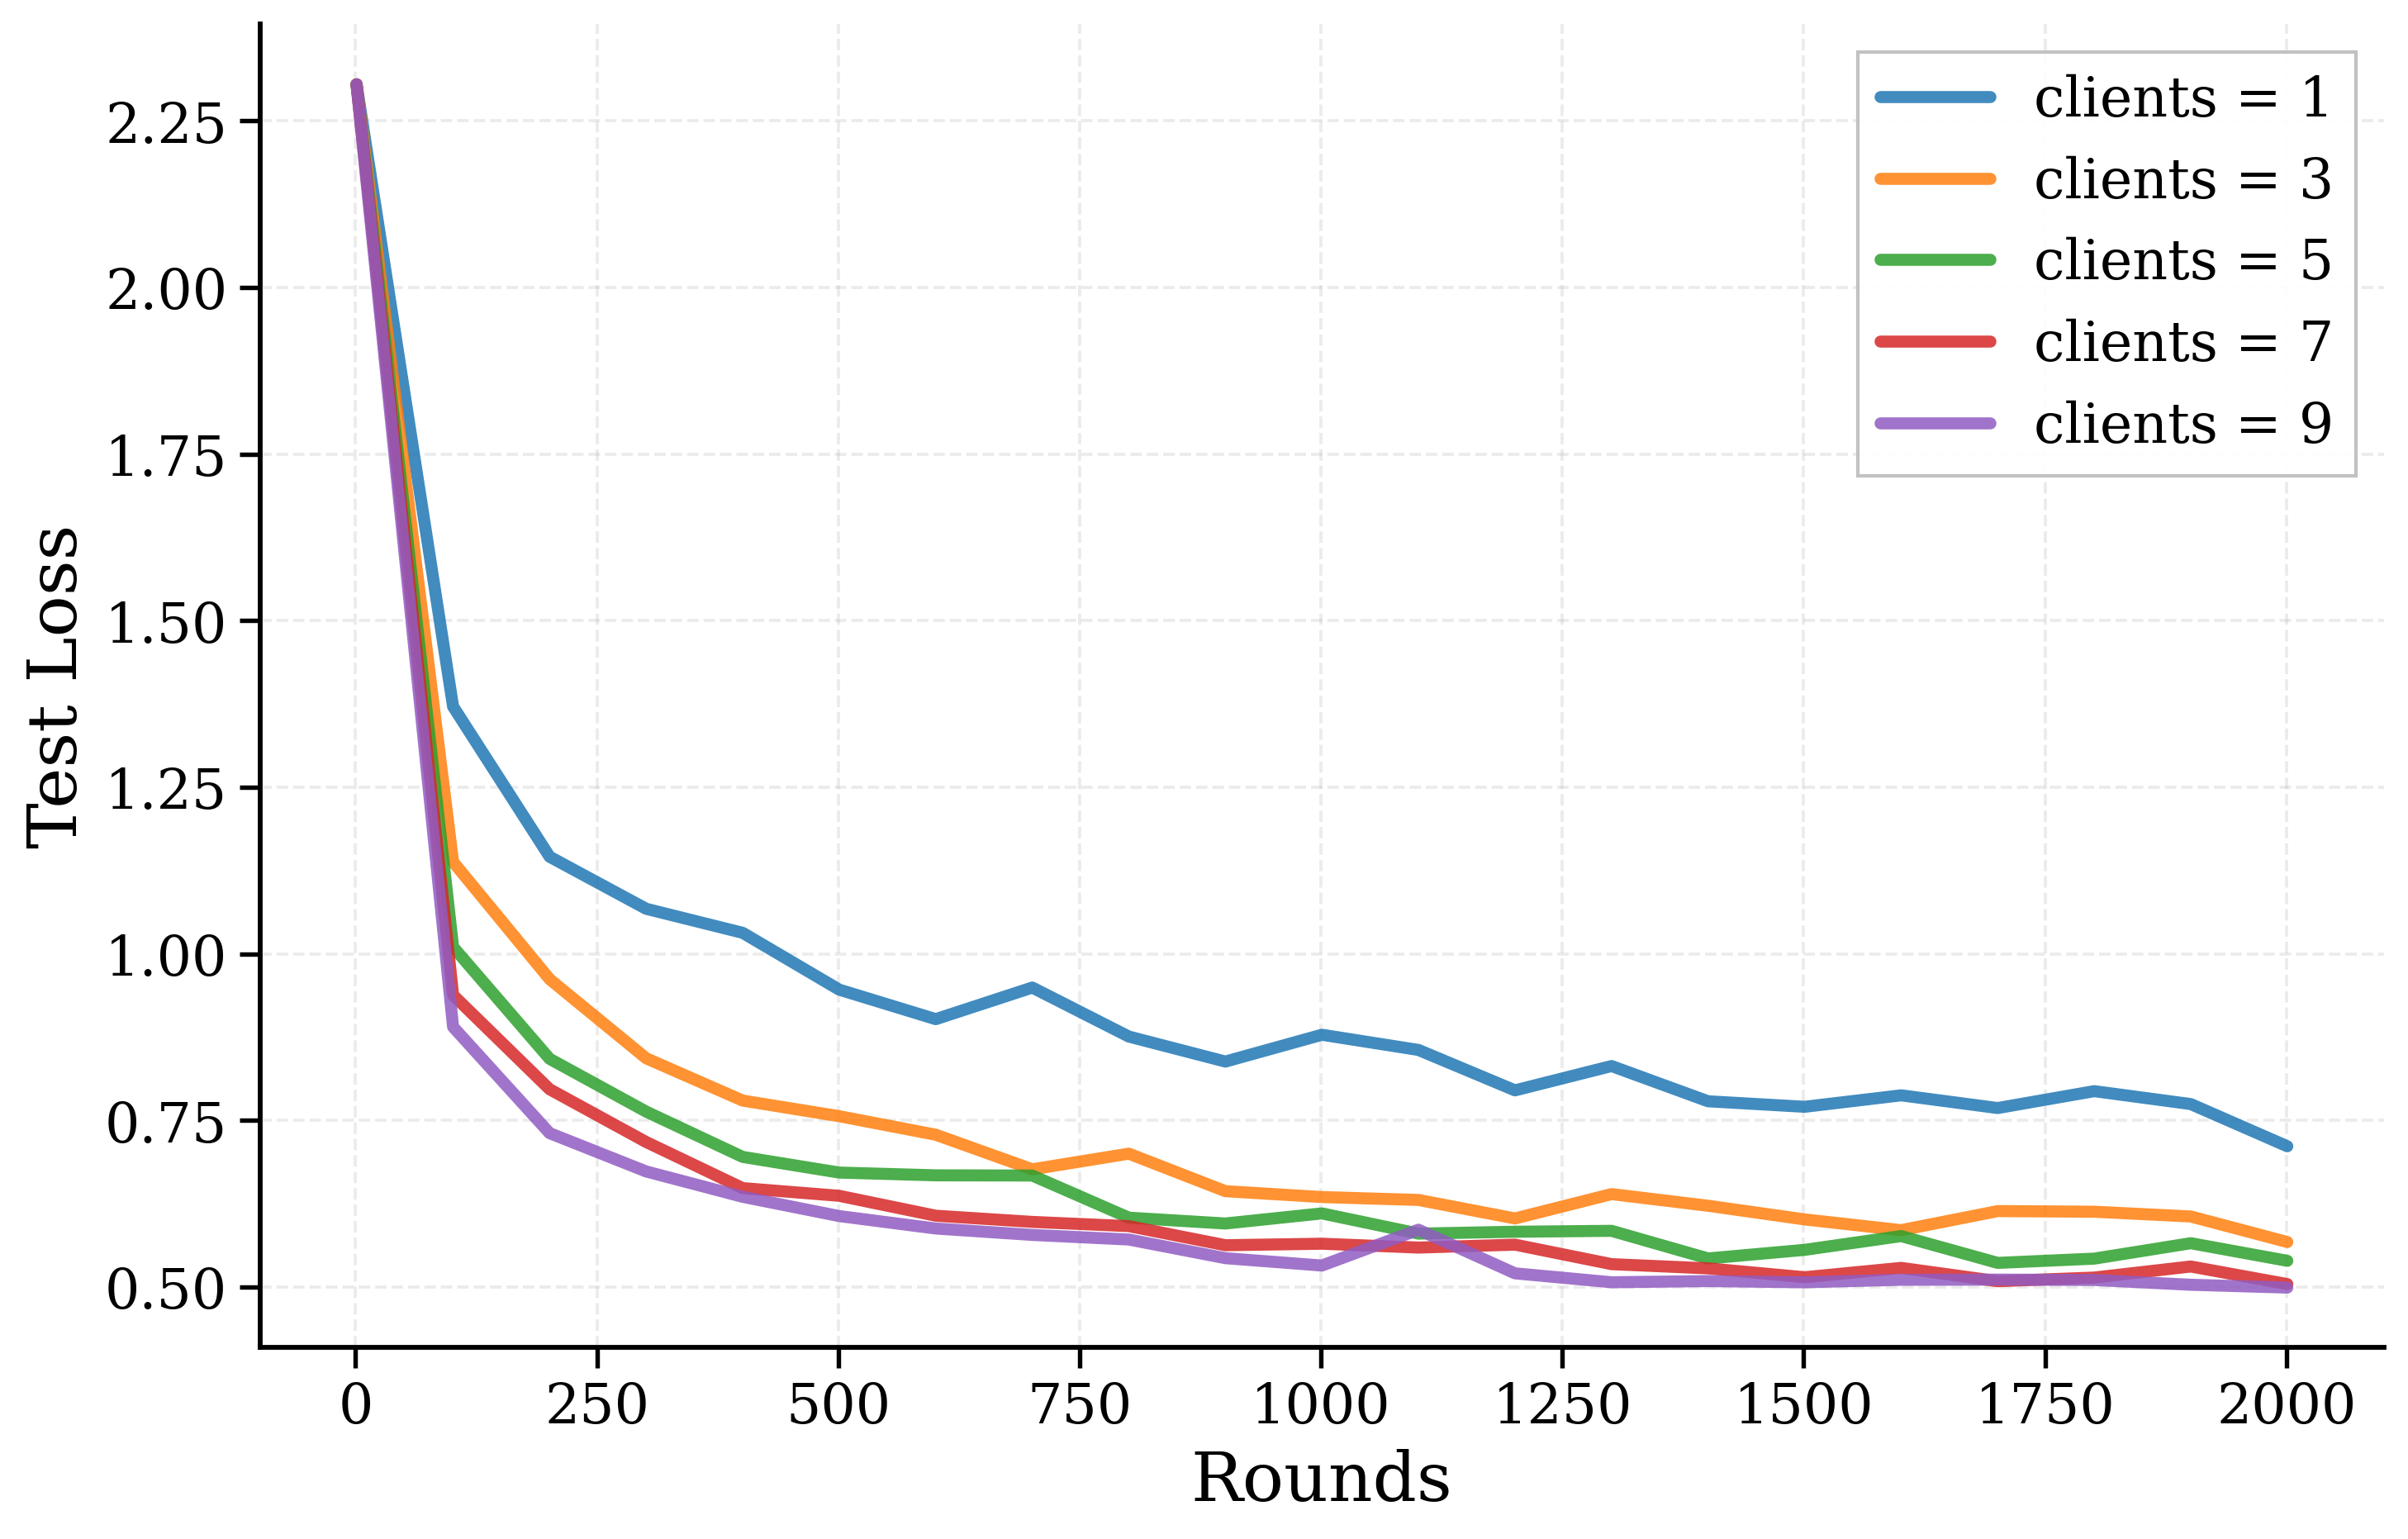
\includegraphics[width=\textwidth]{images/federated_images/signmuon_loss.png} 
        \caption{Test Loss}
    \end{subfigure}
    \hfill
    \begin{subfigure}[b]{0.48\textwidth}
        \centering
        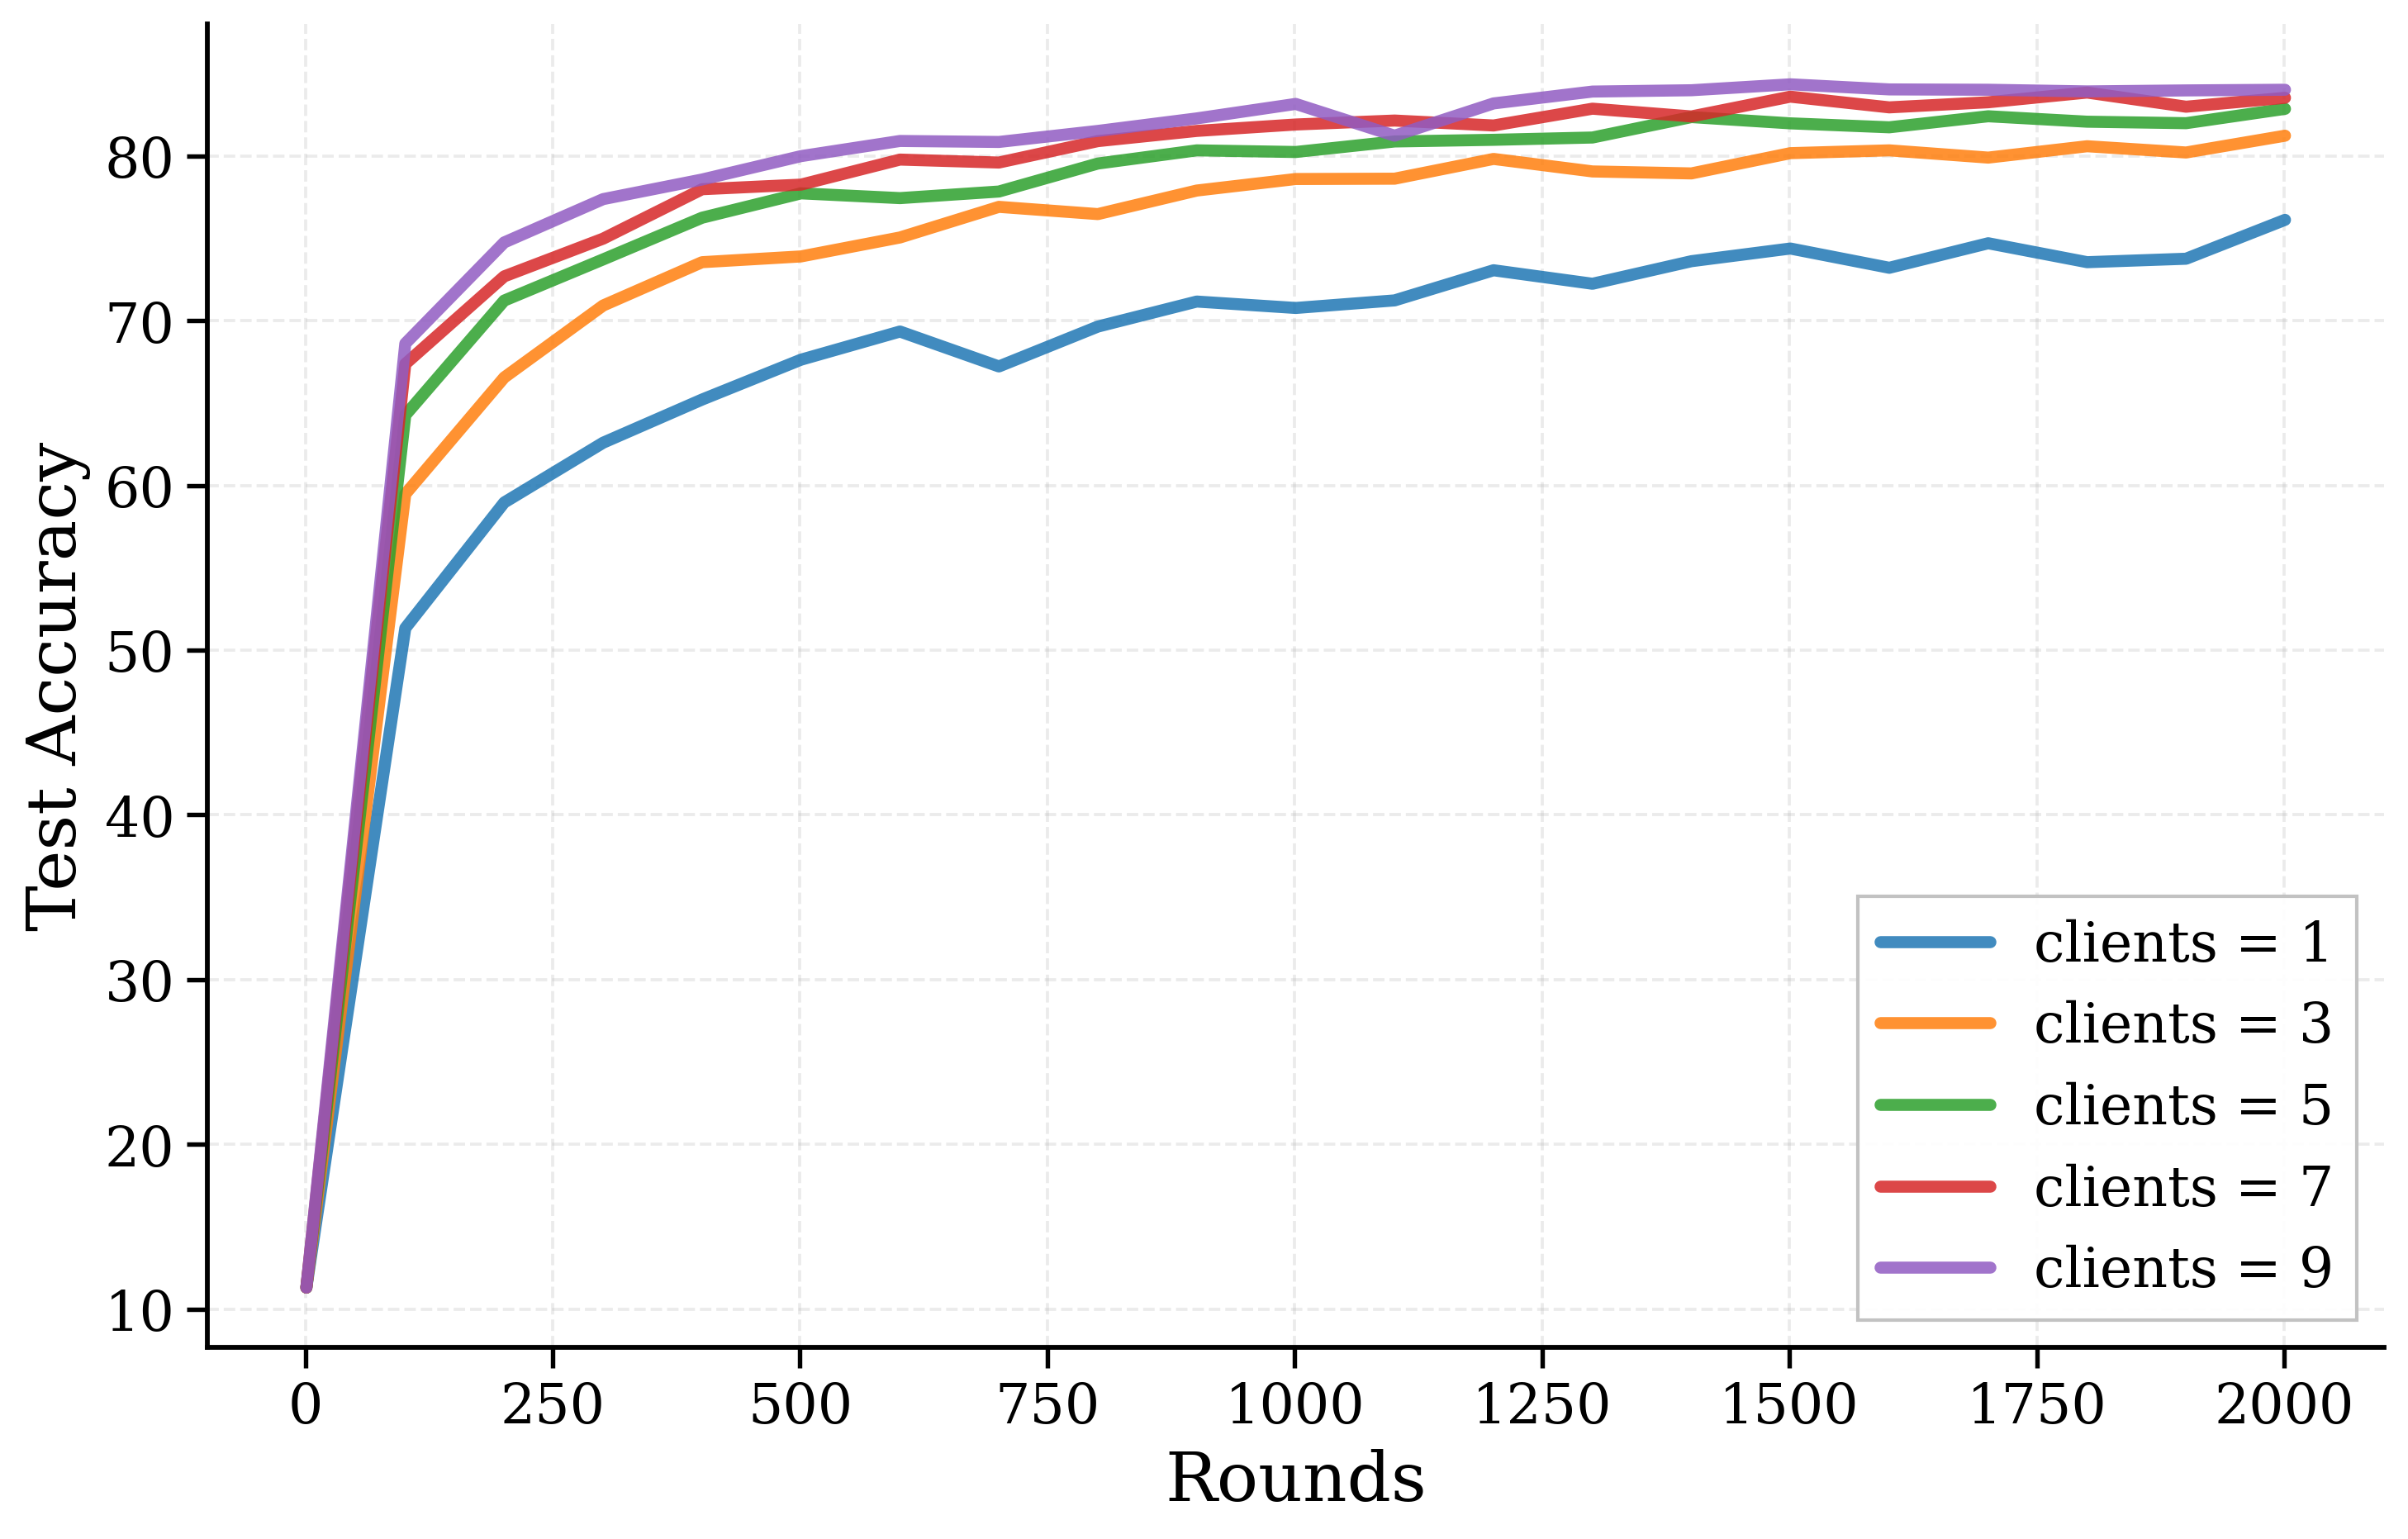
\includegraphics[width=\textwidth]{images/federated_images/signmuon_acc.png}
        \caption{Test Accuracy}
    \end{subfigure}
    \caption{CIFAR-10 Federated Learning. Experiment 1. Scalability of the SignMuon Algorithm.}
    \label{fig:exp_1}
\end{figure}


\subsection{Federated training results. Experiment 2}\label{app:results_fed:2}
\begin{table}[H]
\centering
\caption{CIFAR-10 Federated Learning. Experiment 2: Comparison of Optimization Algorithms with (N = 3) Clients.}
\label{tab:exp_2}
\small
\renewcommand{\arraystretch}{1.2}
\begin{tabular}{|c|c|c|c|c|c|c|c|c|}
\hline
\textbf{Dataset} & \textbf{Optimizer} & \textbf{Rounds} & \textbf{Clients} & \textbf{Steps} & \textbf{Batch} & \textbf{LR} & \textbf{Mom} & \textbf{Test Acc} \\
\hline
\multirow{6}{*}{CIFAR-10} & SignMuon & \multirow{6}{*}{2000} & \multirow{6}{*}{3} & \multirow{6}{*}{1} & \multirow{6}{*}{64} & 0.001 & \multirow{6}{*}{0.9} & 81.24\% \\
\cline{2-2} \cline{7-7} \cline{9-9}
 & Muon & & & & & 0.05 & & 81.27\% \\
\cline{2-2} \cline{7-7} \cline{9-9}
 & SignSGD & & & & & 0.001 & & 65.96\% \\
\cline{2-2} \cline{7-7} \cline{9-9}
 & SGD & & & & & 0.03 & & 76.77\% \\
\cline{2-2} \cline{7-7} \cline{9-9}
 & Adam & & & & & 0.001 & & 70.83\% \\
\cline{2-2} \cline{7-7} \cline{9-9}
 & EF-USignMuon & & & & & 0.02 & & 80.69\% \\
\hline
\end{tabular}
\end{table}

\begin{figure}[H]
    \centering
    \begin{subfigure}[b]{0.48\textwidth}
        \centering
        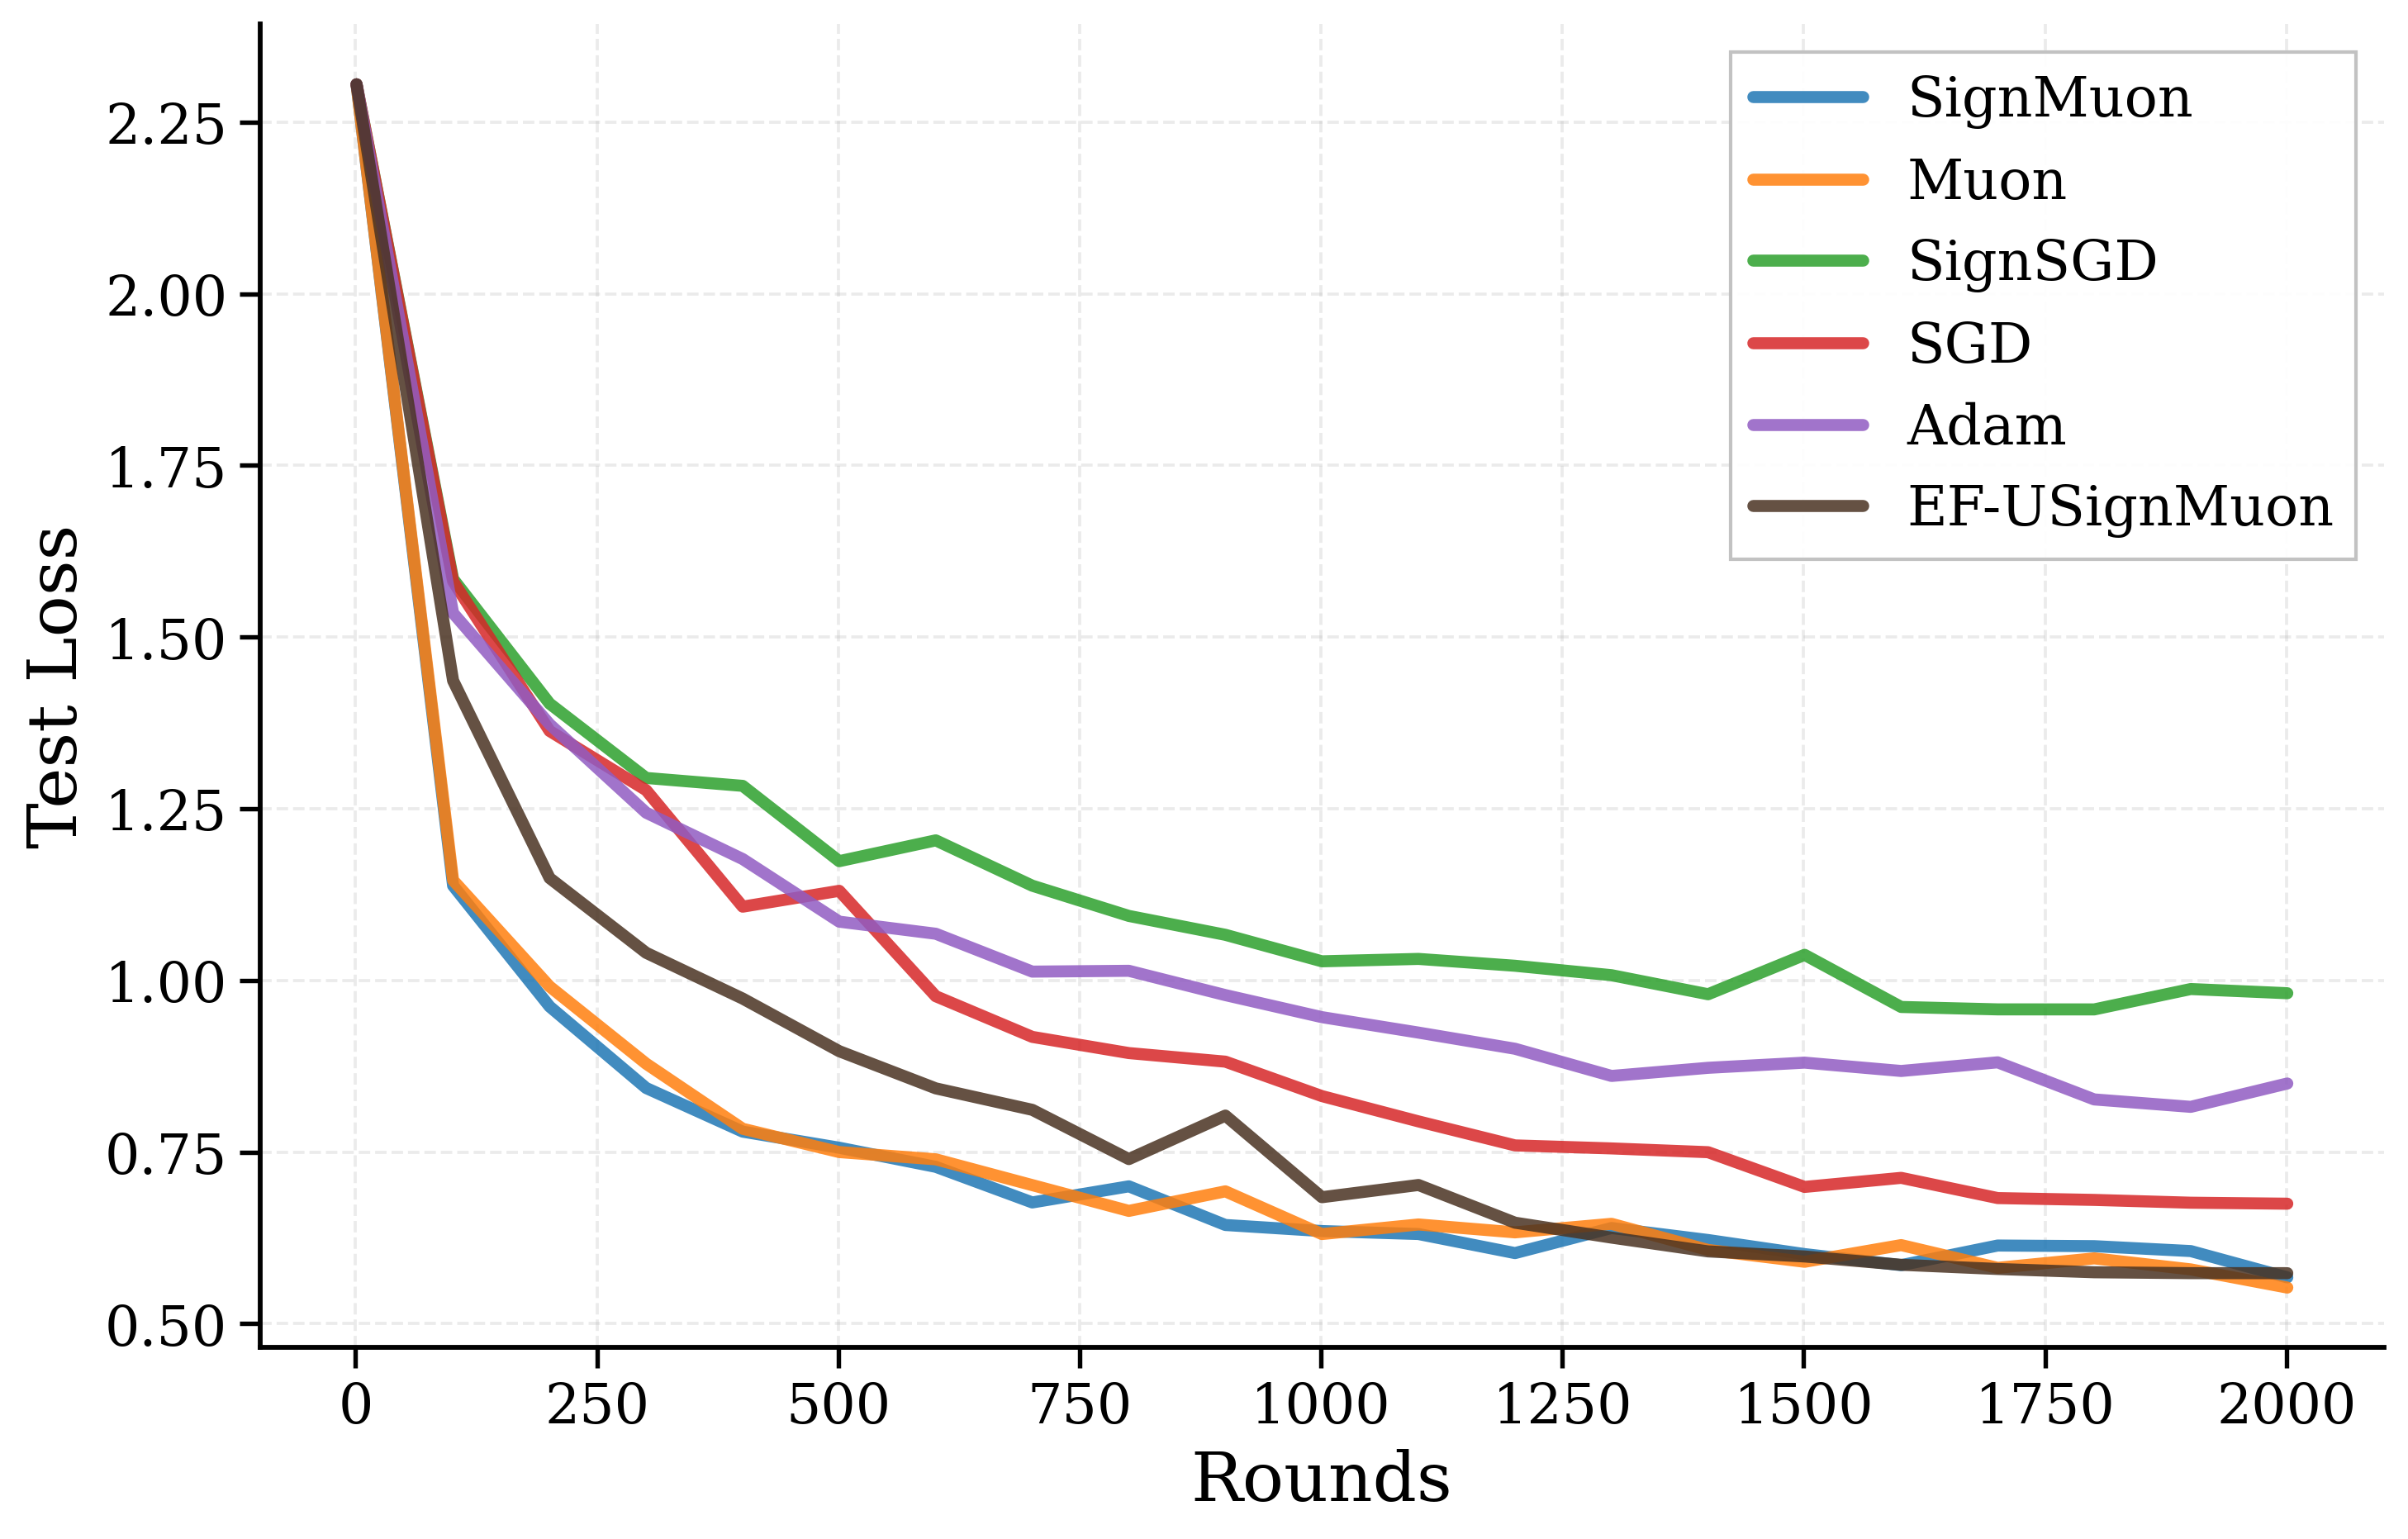
\includegraphics[width=\textwidth]{images/federated_images/3_1_loss.png} 
        \caption{Test Loss}
    \end{subfigure}
    \hfill
    \begin{subfigure}[b]{0.48\textwidth}
        \centering
        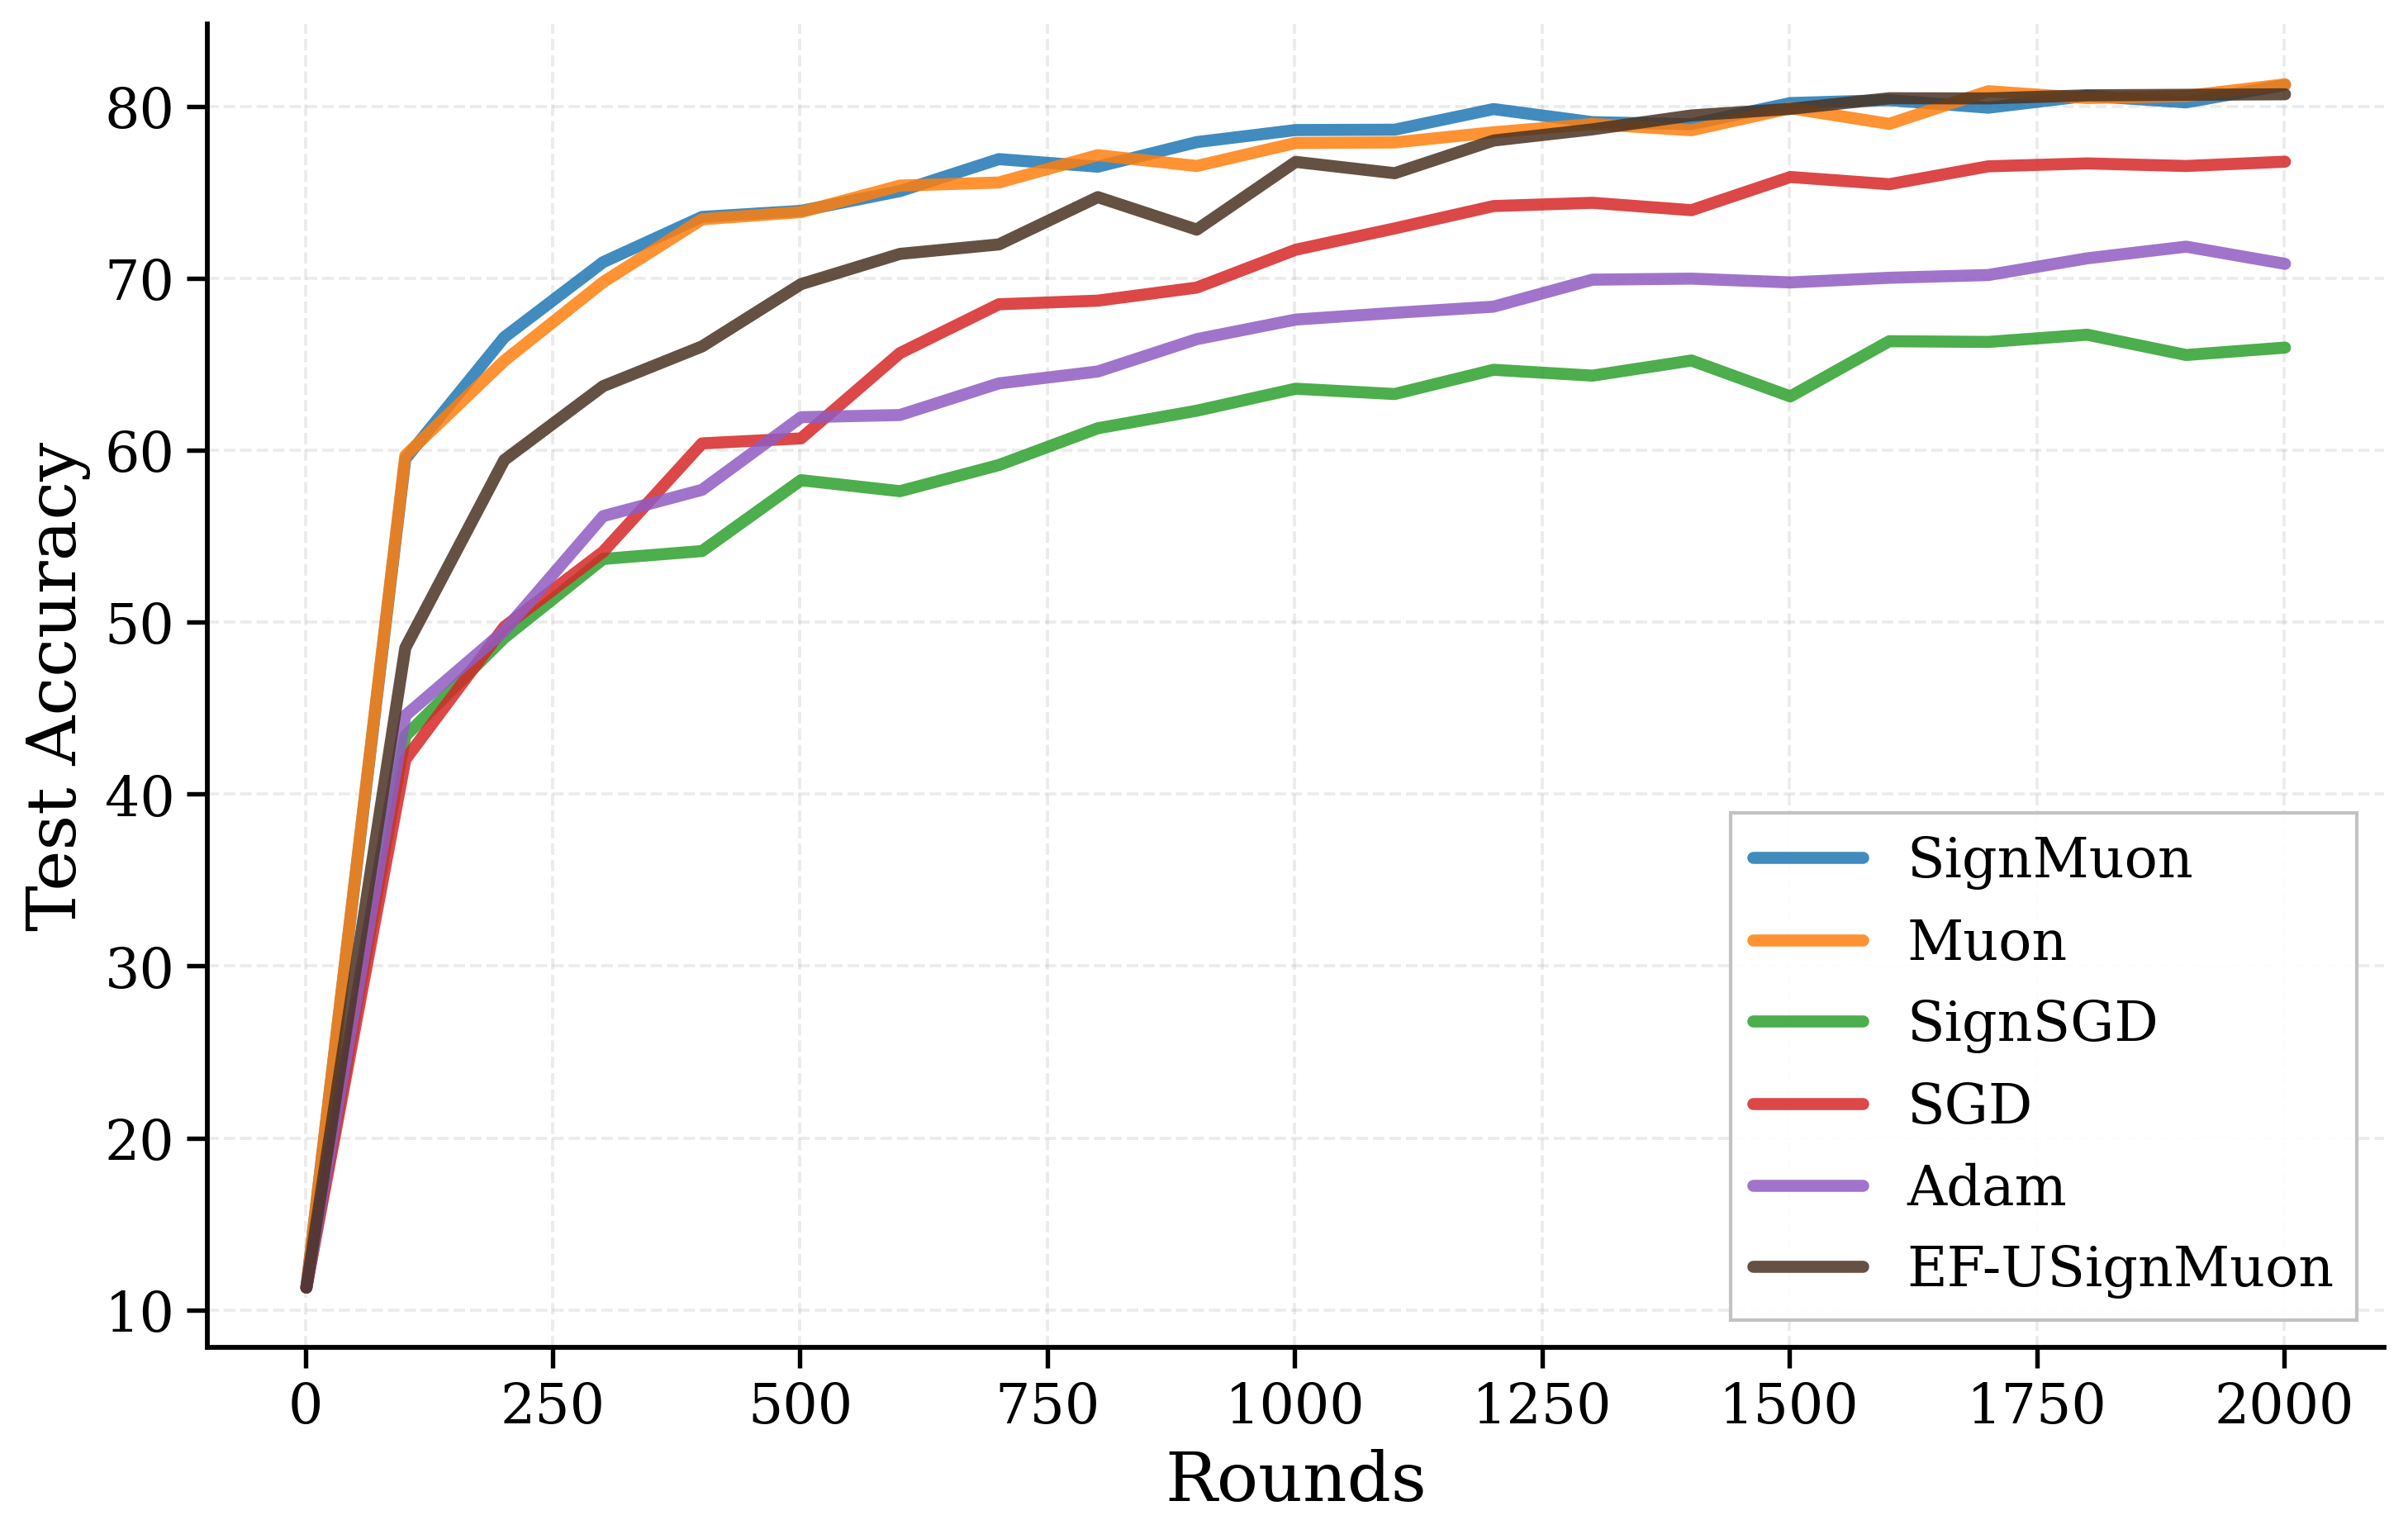
\includegraphics[width=\textwidth]{images/federated_images/3_1_acc.png}
        \caption{Test Accuracy}
    \end{subfigure}
    \caption{CIFAR-10 Federated Learning. Experiment 2: Comparison of Optimization Algorithms with (N = 3) Clients.}
    \label{fig:exp_2}
\end{figure}

\subsection{Federated training results. Experiment 3}\label{app:results_fed:3}
\begin{figure}[H]
    \centering
    \begin{subfigure}[b]{0.48\textwidth}
        \centering
        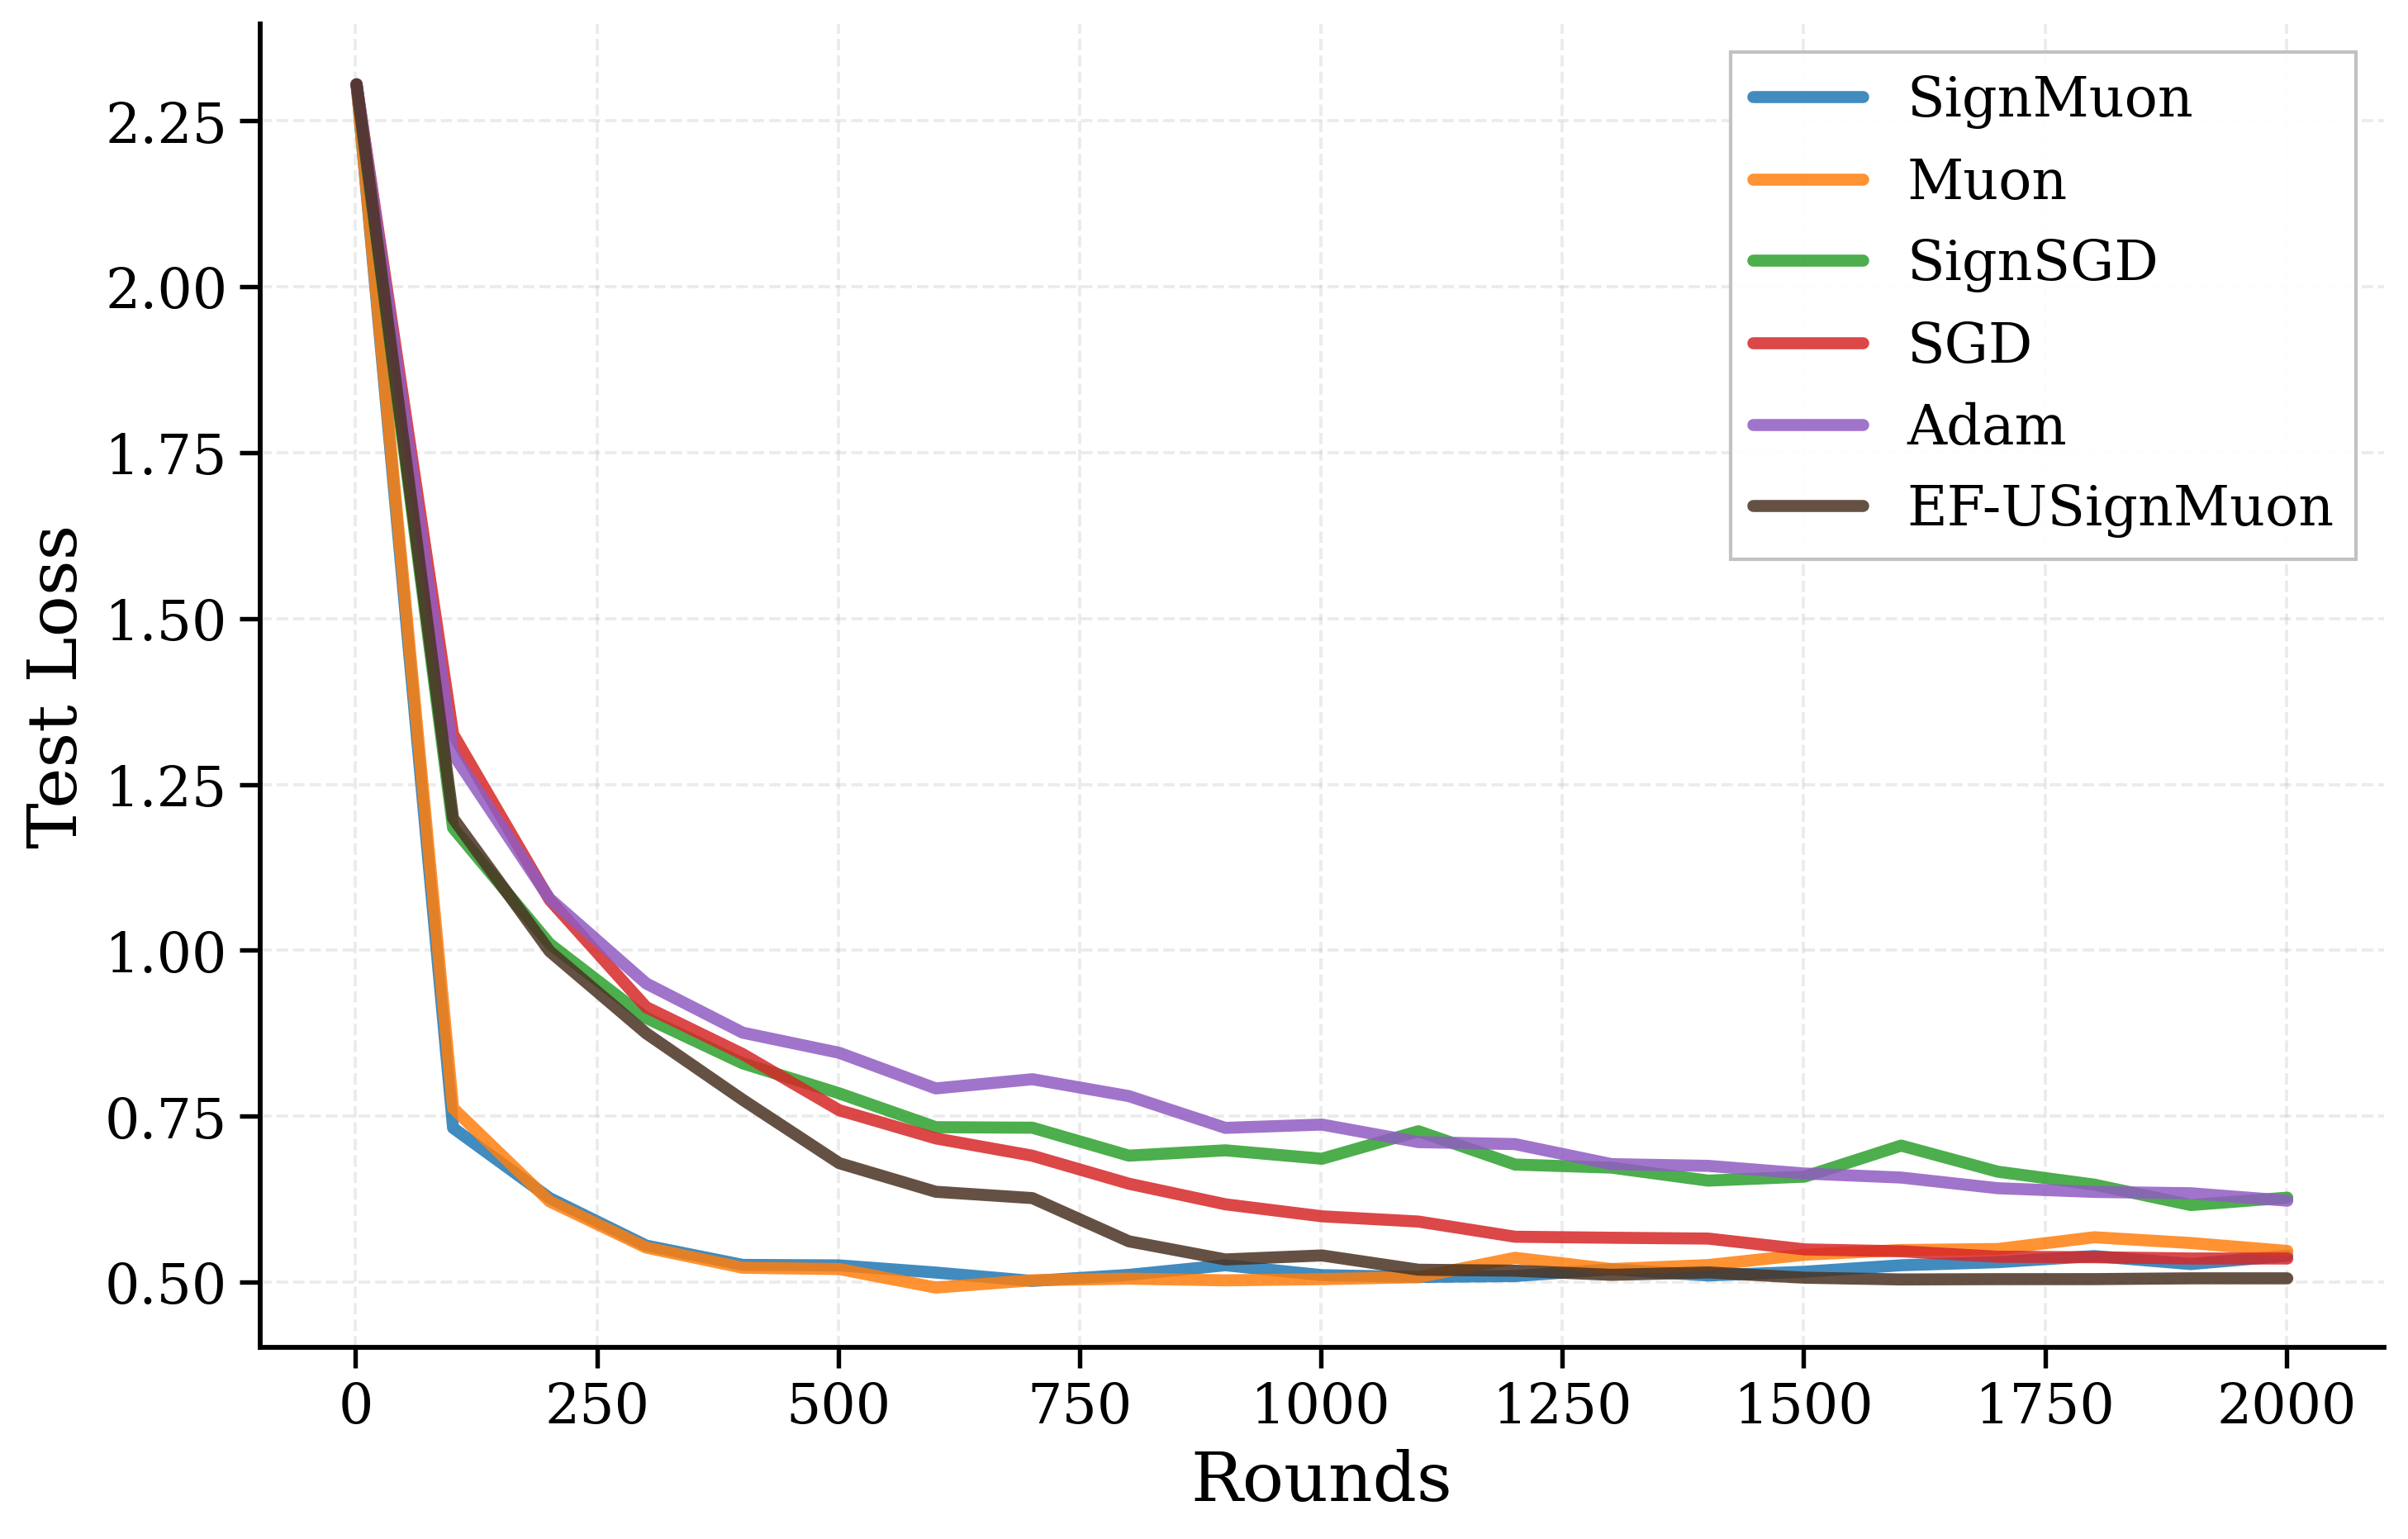
\includegraphics[width=\textwidth]{images/federated_images/10_3_loss.png} 
        \caption{Test Loss}
    \end{subfigure}
    \hfill
    \begin{subfigure}[b]{0.48\textwidth}
        \centering
        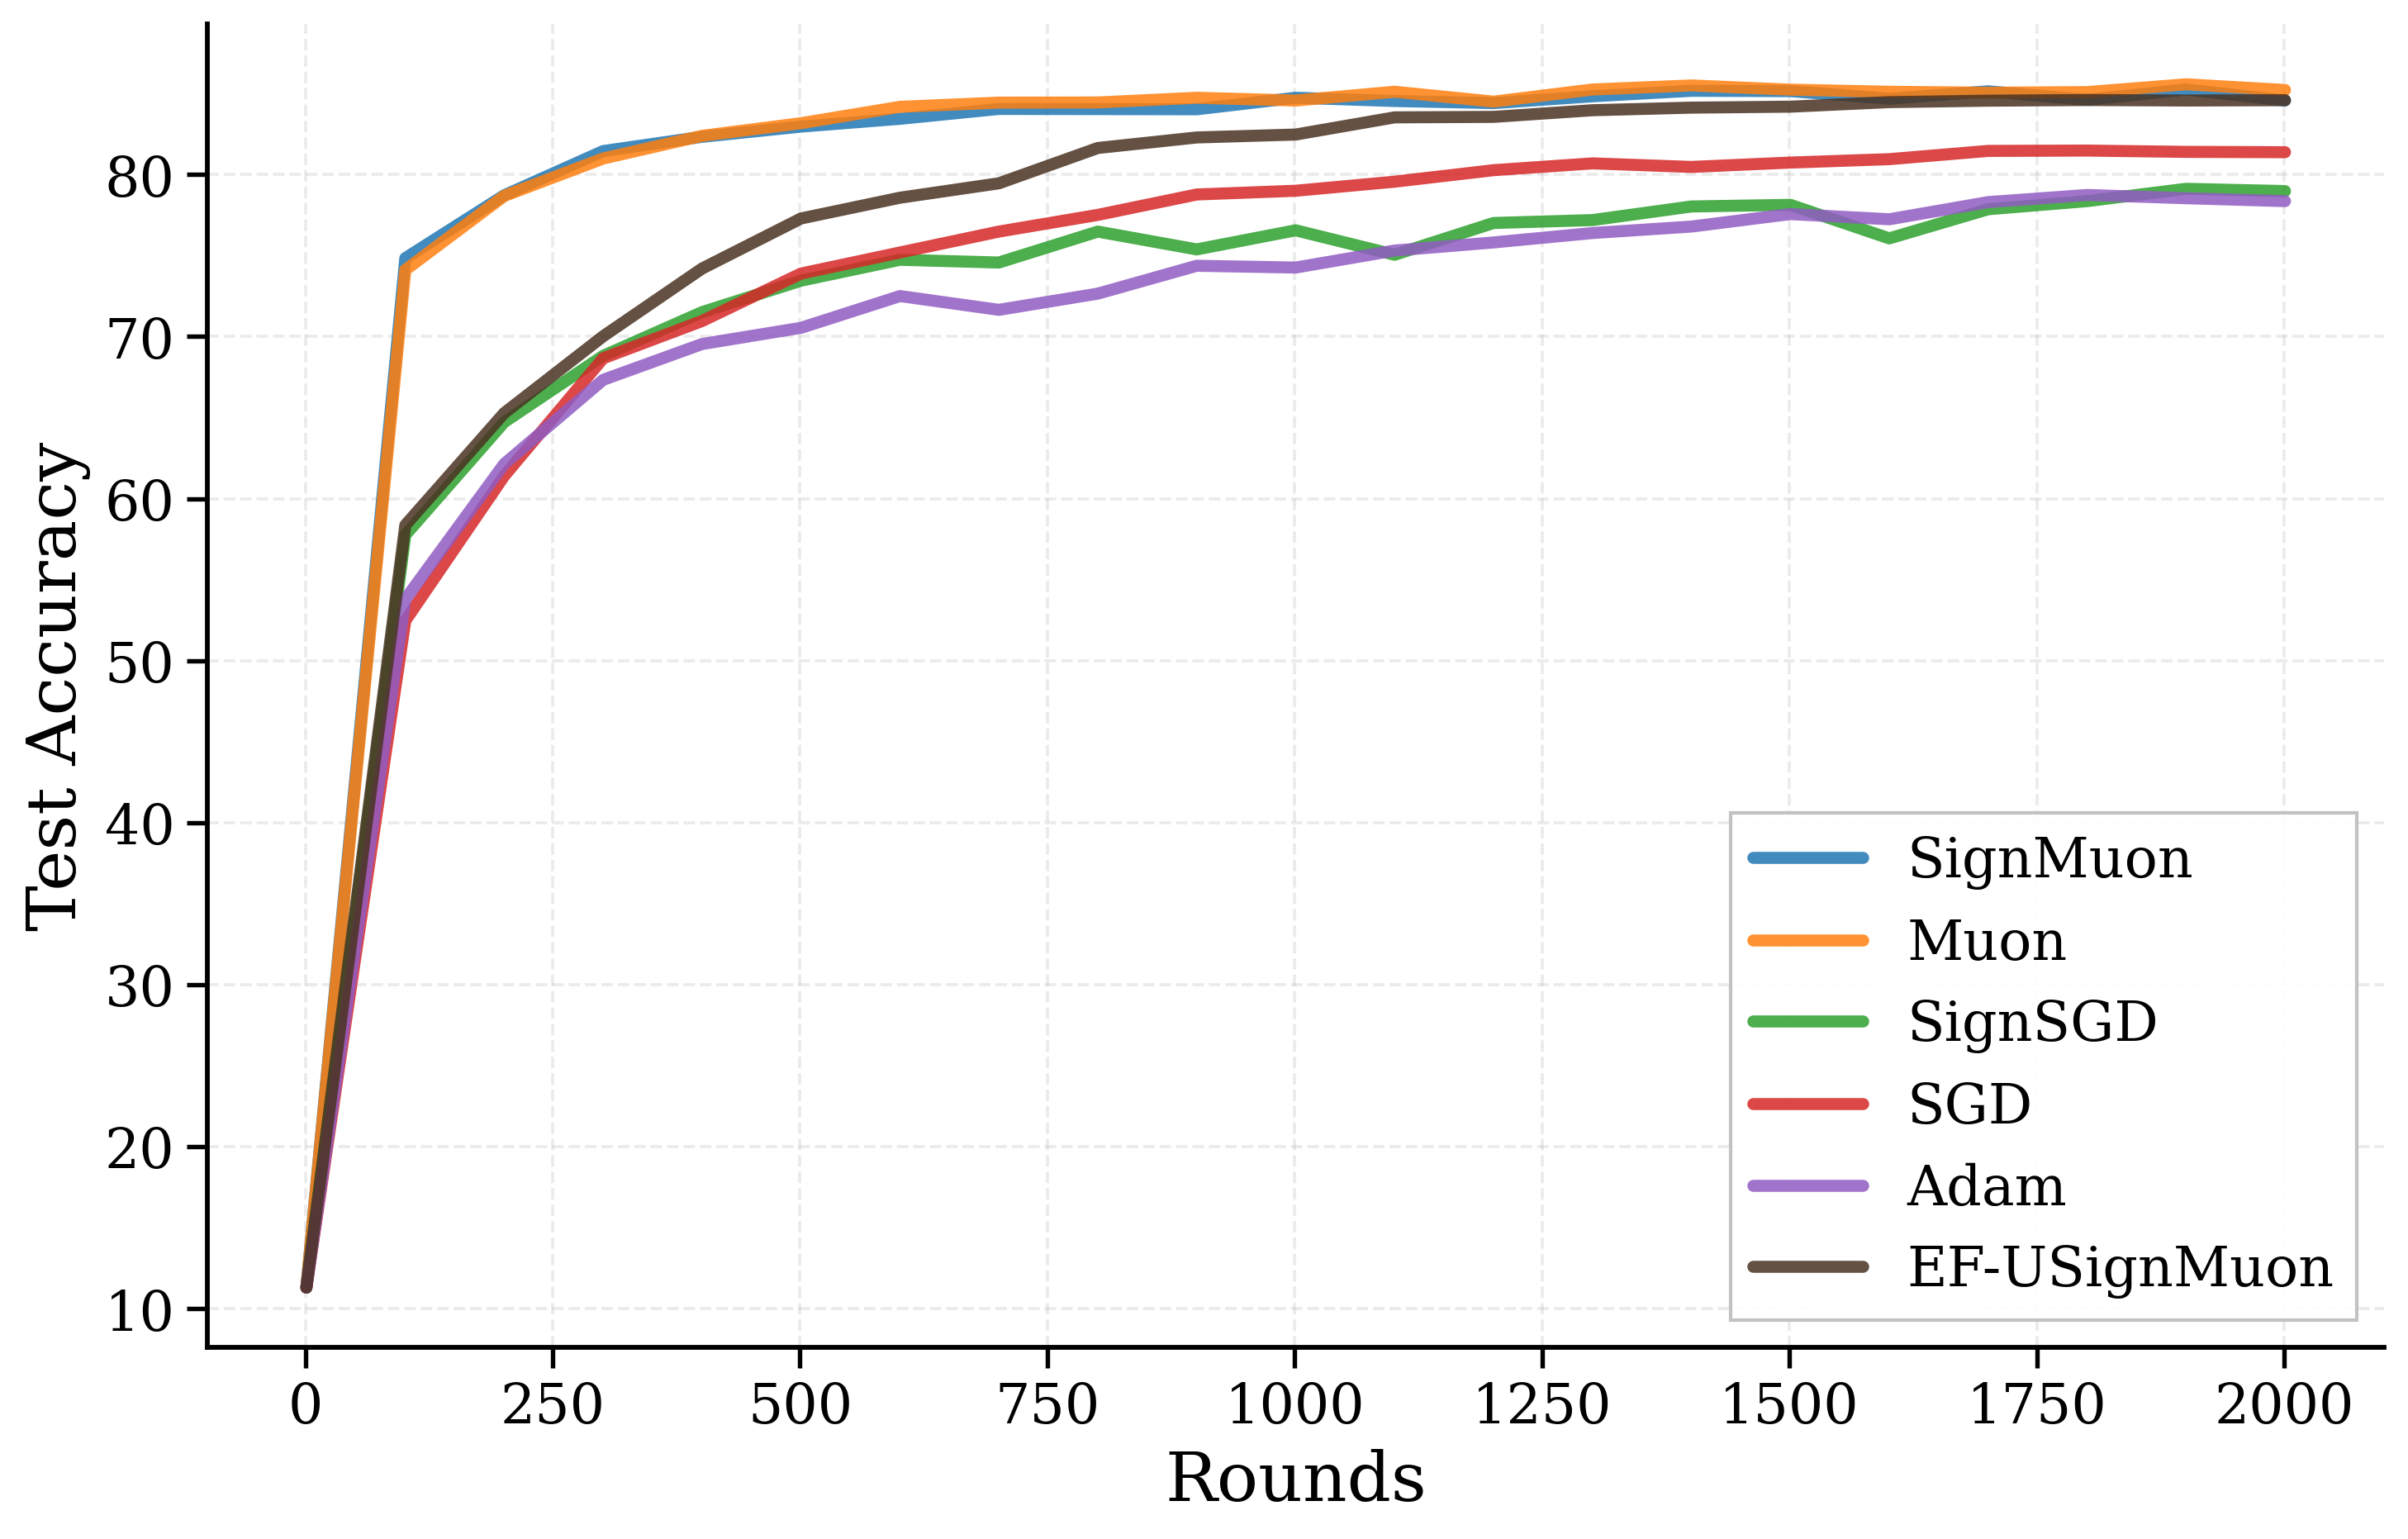
\includegraphics[width=\textwidth]{images/federated_images/10_3_acc.png}
        \caption{Test Accuracy}
    \end{subfigure}
    \caption{CIFAR-10 Federated Learning. Experiment 3: Comparison of Optimization Algorithms with (N = 10) Clients.}
    \label{fig:exp_3}
\end{figure}


\end{document}